\apendice{Plan de Proyecto Software}

\section{Introducción}

Este apartado presenta, en primer lugar, la planificación temporal seguida durante el desarrollo, desglosando el proyecto en tareas e hitos y estableciendo su evolución cronológica. Para ello, se adopta un enfoque iterativo e incremental inspirado en metodologías ágiles, particularmente \textit{Scrum}, organizando el trabajo en ciclos cortos llamados \textit{Sprints} con los que se busca conseguir una correcta revisión del progreso y una posible adaptación ante incidencias o cambios de alcance, manteniendo una visión continua del conjunto de tareas pendientes y completadas mediante el denominado \textit{Product Backlog}, que funciona como un registro de las labores a llevar a cabo.

Finalmente, el plan se completa con un estudio de viabilidad que analiza el proyecto desde una perspectiva económica y legal. En esta parte se consideran los costes asociados al desarrollo y despliegue, así como las implicaciones derivadas del uso de herramientas, librerías y recursos de terceros, prestando especial atención a licencias software y condiciones de uso, con el objetivo de asegurar que la solución propuesta sea sostenible, reutilizable y coherente con un escenario de explotación real.

\section{Planificación temporal}
En este apartado se recoge la evolución del trabajo desarrollado a lo largo de los distintos \textit{sprints}, indicando para cada uno de ellos el periodo temporal correspondiente, los objetivos planteados, la dedicación estimada y real, así como las principales tareas llevadas a cabo. Esta organización permite reflejar de forma ordenada el avance efectivo del proyecto y la manera en que se fueron cerrando, ajustando o replanificando distintos bloques de trabajo conforme la aplicación y la memoria evolucionaban.

Durante los primeros \textit{sprints} del proyecto, la planificación y el seguimiento no se estructuraron todavía mediante una estimación homogénea en \textit{points}, sino principalmente a partir de horas previstas y tareas registradas de forma más informal. Como consecuencia, en esta fase inicial no fue posible generar \textit{burndown reports} consistentes ni comparables, ya que la organización del trabajo todavía no seguía un criterio de medición suficientemente estable. Por este motivo, los \textit{burndown reports} solo se incorporan a partir del \textit{Sprint~8}, momento en el que la planificación ya estaba mejor consolidada y permitía representar de forma más fiel la evolución de los \textit{open points} a lo largo de cada iteración.

\subsection{Sprint 1 - Documentación e investigación de conceptos teóricos}
El \textit{Sprint} 1 se desarrolló del 25 de octubre al 7 de noviembre. En esta primera etapa, antes del inicio del segundo semestre, los \textit{sprints} estaban pensados para una duración de dos semanas, y funcionó como una toma de contacto inicial con el TFG, ya que comencé a trabajar en él antes de lo establecido oficialmente: aunque la asignatura la curso en el segundo semestre, empecé a avanzar a finales del primero. Además, la semana siguiente a iniciar el TFG comencé mis prácticas en empresa y, junto con tres asignaturas en paralelo, me resultó complicado reservar horas estables para esta tarea, aunque fui sacando tiempo progresivamente.

Para este \textit{sprint} estimé una dedicación total de 22~horas. Finalmente, dediqué aproximadamente 15~horas, lo que se reflejó en que no llegué a completar todas las \textit{issues} previstas.

Las tareas planteadas para este \textit{sprint} fueron:
\begin{itemize}
	\item Documentación e investigación de conceptos teóricos asociados al proyecto (segmentación semántica, predicción densa, aprendizaje profundo, evaluación y métricas, \textit{encoders} y modelos/arquitecturas).
	\item Estudio en detalle del artículo base sobre el que se apoya el TFG, para comprender su fundamentación teórica y el enfoque metodológico.
	\item Localización y recopilación de bibliografía para los distintos conceptos a documentar.
	\item Configuración del repositorio y del flujo de trabajo: GitHub, operación remota y entorno de desarrollo en VS Code.
	\item Puesta en marcha del entorno \LaTeX{} con la plantilla proporcionada por los profesores y configuración de herramientas (\TeX{}studio, MiK\TeX{} Console y \TeX{}works).
	\item Selección y configuración de la herramienta de gestión de tareas, optando por Zube.io tras descartar ZenHub.
\end{itemize}

Durante la primera semana me centré principalmente en asentar el entorno de trabajo. Configuré GitHub y el acceso para operación remota, dejé preparado VS Code para trabajar con comodidad y monté la plantilla de \LaTeX{} proporcionada por los profesores. En paralelo, instalé y ajusté las herramientas necesarias para editar y compilar el proyecto, \textit{\TeX{}studio}, \textit{MiK\TeX{} Console} y \textit{\TeX{}works}, ya que al principio necesitaba entender bien cómo organizar el proyecto y compilar sin fricción. También exploré opciones para la gestión del tablero de trabajo: tras comprobar que ZenHub me daba un error inesperado y sin mucha posibilidad de solución, migré a Zube.io y dejé preparada la estructura para organizar las \textit{issues}.

A lo largo de las dos semanas, la parte principal del \textit{sprint} fue la investigación y búsqueda bibliográfica. Dediqué la mayor parte del tiempo a leer y estudiar diferentes \textit{papers} científicos para asentar la base teórica, especialmente el artículo principal en el que se fundamenta el TFG, que trabajé en detalle para comprender correctamente su planteamiento. Como resultado de esta fase, conseguí recopilar bibliografía para la mayoría de los conceptos que tenía previstos documentar, aunque la redacción completa no llegó a cerrarse en este \textit{sprint}.

En cuanto a la documentación escrita, el objetivo era redactar las \textit{issues} de conceptos teóricos planificadas; sin embargo, por falta de tiempo y por la incertidumbre inicial sobre cómo estructurar el contenido, únicamente avancé en la redacción de dos bloques: la definición de \textit{Visión por Computador} y los conceptos teóricos generales de la \textit{Segmentación Semántica}. Además, estos avances no quedaron consolidados mediante \textit{commit} hasta el \textit{sprint} siguiente, ya que durante este primer tramo estuve reorganizando la estructura del proyecto y me costó definir correctamente las bases del mismo.

\subsection{Sprint 2 - Primer prototipo de la aplicación web}
El \textit{Sprint} 2 abarcó del 8 de noviembre al 22 de noviembre. Para este periodo estimé una dedicación de 12,5~horas, aunque finalmente empleé 21~horas. En este punto, la planificación todavía se encontraba en una fase inicial de ajuste, por lo que el seguimiento del trabajo seguía haciéndose de forma poco estructurada y no mediante una estimación estable en \textit{points}. En su lugar, intenté organizarme con un campo personalizado de \textit{horas}, pero comprobé que no resultaba útil para medir progreso ni para generar informes de seguimiento.

Los objetivos principales de este \textit{sprint} fueron los siguientes:
\begin{itemize}
	\item Estudiar la documentación oficial de Flask y realizar los tutoriales propuestos~\cite{flask_user_guide}.
	\item Diseñar el \textit{mockup} inicial de la aplicación web.
	\item Implementar una primera versión sencilla de la web, con cuatro botones principales.
	\item Verificar el flujo de entrada/salida de la aplicación: recibir una imagen en Flask y dibujar en HTML unas líneas de esquina a esquina sobre la imagen.
	\item Añadir documentación del código y una primera batería de \textit{tests} asociados a este acercamiento inicial.
\end{itemize}

Durante la primera semana me centré en dos frentes. Por un lado, diseñé el \textit{mockup} de la web para fijar la estructura de pantallas y el flujo esperado de uso. Por otro, dediqué tiempo a estudiar Flask, siguiendo la documentación oficial y completando los tutoriales, ya que necesitaba asentar la base del \textit{backend} antes de comenzar con una implementación funcional.

En la segunda semana abordé la implementación inicial de la aplicación. Construí un prototipo sencillo con los cuatro botones definidos y dejé operativo el flujo mínimo: la aplicación recibía una imagen en el servidor y se mostraba en el \textit{frontend} con un trazado simple de líneas de esquina a esquina. Este paso fue clave para validar de forma temprana el formato del JSON de trazas y confirmar que el intercambio de datos entre \textit{backend} y \textit{frontend} estaba funcionando como esperaba. Además, documenté el código y añadí \textit{tests} básicos para asegurar que este acercamiento inicial quedaba mínimamente cubierto.

A lo largo del \textit{sprint} también intenté avanzar en la redacción de conceptos teóricos arrastrados del \textit{sprint} anterior, pero apenas conseguí progresar en esa parte debido a la carga de trabajo asociada a la puesta en marcha del prototipo. Aun así, logré completar las tareas específicas definidas para este \textit{sprint}. La única excepción fue la integración del \textit{mockup} en la memoria, que no pude dejar lista a tiempo por un fallo en la configuración del entorno de \LaTeX{} en \TeX{}studio, lo que obligó a posponer esa incorporación.

\subsection{Sprint 3 - Ajustes en estilo y aplicación de la web}
El \textit{Sprint} 3 se desarrolló entre el 22 de noviembre y el 6 de diciembre. Para este \textit{sprint} estimé inicialmente 4,5~horas, ya que en ese momento todavía no estaba creando todas las tareas de forma consistente y únicamente llegué a registrar algunas. Sin embargo, la dedicación real fue notablemente superior, alcanzando aproximadamente 18~horas, debido a que se fueron abriendo frentes adicionales de revisión y ajuste conforme avanzaba el prototipo.

Cabe destacar que, durante la reunión que dio inicio al \textit{sprint}, conocí al que sería mi otro tutor del TFG, David Martínez, quien me orientó sobre varios aspectos relacionados con el estilo de la interfaz, como Bootstrap, Tailwind y alternativas, y sobre ciertos requerimientos esperables en la web, lo que condicionó parte de las decisiones técnicas de este periodo.

Los objetivos abordados durante este \textit{sprint} fueron los siguientes:
\begin{itemize}
	\item Sustituir el botón de dibujar trazas por un \textit{checkbox}, simplificando el flujo de interacción.
	\item Corregir la funcionalidad asociada al PNG, de forma que la web dibujase las trazas sobre el mismo PNG original en lugar de generar un PNG nuevo.
	\item Investigar Bootstrap y TailwindCSS, y elaborar una comparativa entre ambos enfoques.
	\item Estudiar y preparar la adopción de DaisyUI como capa de componentes sobre Tailwind.
	\item Realizar limpieza del código, mejorar su documentación y aplicar pequeños ajustes locales para verificación de versiones.
	\item Continuar, de forma paralela, con la investigación teórica y la recopilación bibliográfica de conceptos arrastrados del \textit{sprint} 1.
\end{itemize}

Durante los primeros días me centré en mejorar el prototipo existente y en cerrar cambios funcionales pequeños pero importantes. En primer lugar, sustituí el botón dedicado a dibujar trazas por un \textit{checkbox}, ya que resultaba más coherente con el tipo de acción y evitaba pasos innecesarios en el uso. En paralelo, corregí la funcionalidad asociada al PNG: hasta ese momento, mi aproximación consistía en generar un archivo nuevo con las trazas, pero el comportamiento esperado era que la aplicación dibujase directamente sobre el mismo PNG que se estaba visualizando. Este cambio fue relevante porque simplificó el flujo de representación y alineó la salida con el objetivo de validación visual de las trazas.

Además, en esta primera semana dediqué tiempo a investigar y comparar Bootstrap y TailwindCSS, con el objetivo de entender qué enfoque se ajustaba mejor a una interfaz sencilla pero mantenible. Como resultado, dejé documentada una comparativa que me permitió aclarar las diferencias entre un \textit{framework} basado en componentes predefinidos (Bootstrap) y uno basado en utilidades (Tailwind), teniendo en cuenta el grado de personalización, la curva de aprendizaje y el impacto en el mantenimiento del proyecto. Estos cambios quedaron reflejados junto con una primera limpieza y documentación del código, de forma que el prototipo quedase más legible de cara a iteraciones posteriores.

En la segunda semana el foco pasó a DaisyUI. Dediqué tiempo a estudiar este conjunto de componentes sobre Tailwind, explorando su filosofía y la forma de integrarlo en un proyecto web, ya que la idea era disponer de componentes consistentes sin perder la flexibilidad de Tailwind. En este proceso también realicé algunos ajustes locales para verificación de versiones y reorganicé parte del proyecto eliminando dependencias que no estaban aportando valor en ese momento, con la intención de reducir complejidad antes de iniciar una migración estética más profunda.

Por último, durante todo el \textit{sprint} mantuve un trabajo paralelo de investigación teórica asociado a conceptos que venía arrastrando del \textit{sprint} 1. Aunque no llegué a consolidar estos avances en \textit{commits} específicos, continué revisando bibliografía y tomando notas sobre bloques pendientes, como, por ejemplo, aspectos relacionados con predicción densa, tipos de arquitecturas y métricas de evaluación, con la intención de retomar su redacción cuando el entorno técnico de la web quedase más estabilizado.

\subsection{Sprint 4 - Navidades}
Antes de iniciar este \textit{sprint}, conviene señalar que del 7 al 19 de diciembre no realicé trabajo enmarcado dentro de un \textit{sprint} como tal, ya que coincidió con el periodo de exámenes y prioricé esa carga académica. En todo caso, si avancé alguna tarea, fue de forma puntual y sin una planificación cerrada.

El \textit{Sprint} 4 abarcó del 19 de diciembre al 9 de enero, coincidiendo en gran medida con el periodo de vacaciones de Navidad. Para este \textit{sprint} estimé una dedicación total de 10~horas, aunque finalmente empleé aproximadamente 24~horas, debido a que aproveché el mayor margen de estas semanas para consolidar decisiones técnicas y recuperar trabajo arrastrado.

Los objetivos principales de este \textit{sprint} fueron los siguientes:
\begin{itemize}
	\item Estudiar y redactar una comparativa entre distintas \textit{engines} posibles para la aplicación y seleccionar una opción final.
	\item Analizar extensiones de bases de datos para VS Code, escoger la alternativa más adecuada y documentar la decisión.
	\item Elaborar el diagrama de casos de uso de la aplicación y documentar los casos asociados.
	\item Recuperar trabajo teórico arrastrado del \textit{sprint} 1, avanzando en la revisión bibliográfica y en la organización de conceptos.
	\item Crear esquemas personales y diagramas de apoyo de flujo y de secuencia para disponer de una referencia visual clara del funcionamiento interno y del estado actual del sistema.
\end{itemize}

En primer lugar, dediqué parte del \textit{sprint} a estudiar y redactar una comparativa entre distintos \textit{engines} que podían utilizarse en la aplicación, analizando sus ventajas e inconvenientes en términos de integración, mantenibilidad y adecuación al flujo previsto. Como resultado de este análisis, pude decantarme por una alternativa concreta y dejar justificadas las razones técnicas de la decisión, de forma que quedase trazabilidad en la memoria.

En paralelo, revisé varias extensiones de bases de datos para VS Code, ya que necesitaba una herramienta práctica para inspeccionar y gestionar el estado de la base de datos durante el desarrollo sin fricción adicional. Tras comparar opciones, seleccioné la que mejor se ajustaba al tipo de base de datos que estaba utilizando y al flujo de trabajo diario, y dejé reflejada la comparativa en la memoria.

Respecto al diagrama de casos de uso, aunque era una tarea planificada para este \textit{sprint}, no llegué a completarlo como entregable final. Sin embargo, avancé una parte importante del trabajo previo: identifiqué y definí los requisitos funcionales del sistema y clarifiqué el alcance de las interacciones principales. Este paso resultó especialmente útil porque me permitió dejar preparado el terreno para, en un \textit{sprint} posterior, transformar esos requisitos en casos de uso formales y documentarlos con un formato consistente.

A pesar de estas tareas planificadas, la parte más relevante del \textit{sprint} fue la consolidación interna del proyecto. Aproveché el periodo de vacaciones para recuperar trabajo del \textit{sprint} 1 que todavía tenía atrasado, principalmente relacionado con la base teórica y la organización de conceptos. Además, elaboré esquemas personales sobre el funcionamiento interno de la aplicación y definí diagramas de flujo y de secuencia iniciales. Este soporte visual me permitió tener una referencia clara del estado del sistema, detectar con mayor facilidad anomalías o incoherencias en el flujo y, en general, orientar mejor las siguientes implementaciones al disponer de un recurso visual estructurado del comportamiento esperado.

\subsection{Sprint 5 - Consolidación de la memoria}
El \textit{Sprint} 5 se desarrolló del 9 al 16 de enero, siendo un \textit{sprint} de una semana. En esta etapa el foco volvió a situarse en la memoria, tanto para corregir redacciones que habían quedado poco pulidas como para recuperar parte de la carga arrastrada desde el \textit{sprint} 1, en ese bloque de conceptos teóricos.

Para este \textit{sprint} estimé un esfuerzo aproximado de 5 \textit{points}. Finalmente, completé un volumen de trabajo equivalente a 18 \textit{points}, ya que, además de los objetivos previstos, aproveché para cerrar tareas heredadas que ya estaban suficientemente encaminadas.

Los objetivos principales de este \textit{sprint} fueron los siguientes:
\begin{itemize}
	\item Revisar y corregir la definición de \textit{Visión por Computador}.
	\item Redactar la introducción del proyecto.
	\item Establecer y redactar los objetivos del trabajo.
	\item Recuperar trabajo pendiente del \textit{sprint} 1 y consolidar conceptos teóricos asociados a arquitecturas de segmentación semántica.
\end{itemize}

A lo largo del \textit{sprint} realicé una revisión general de la memoria, corrigiendo diversos fragmentos que no estaban correctamente redactados y ajustando detalles de estilo para que el texto quedase más homogéneo. En particular, revisé la definición de \textit{Visión por Computador}, reorganizando parte del contenido y refinando la terminología para que fuese más precisa y coherente con el resto del documento.

La mayor parte del tiempo la dediqué a recuperar el trabajo arrastrado del \textit{sprint} 1. En este punto conseguí cerrar por completo el bloque de conceptos relacionado con \textit{Arquitecturas de segmentación semántica}, que era uno de los apartados más extensos y que requería tanto redacción como consolidación de bibliografía. Este avance fue clave porque permitió dejar el capítulo de conceptos teóricos mucho más estable de cara a \textit{sprints} posteriores.

Además, redacté la introducción del proyecto, definiendo el contexto general del TFG y el hilo conductor que seguiría el documento. En paralelo, dejé establecidos los objetivos del trabajo, aunque esta parte no quedó cerrada completamente: la estructura y el contenido principal quedaron definidos, pero el refinamiento final del texto se completaría el primer día del \textit{sprint} siguiente.

Por último, y de forma transversal a todas las tareas anteriores, añadí y ajusté varios textos introductorios en distintas secciones para mejorar la continuidad entre apartados, facilitar la lectura y contextualizar mejor los bloques teóricos antes de entrar en definiciones más específicas.

\subsection{Sprint 6 - Trabajos relacionados y preparación de integración}
El \textit{Sprint} 6 abarcó del 14 al 21 de enero, con una duración de una semana. Para este \textit{sprint} estimé una dedicación total de 18,5~horas, y finalmente empleé 20~horas y 45~minutos.

Los objetivos definidos para este \textit{sprint} fueron los siguientes:
\begin{itemize}
	\item Terminar de redactar los objetivos del trabajo.
	\item Corregir la introducción de la memoria.
	\item Resolver un fallo de compilación en el documento de anexos.
	\item Corregir imágenes de anexos y referencias asociadas.
	\item Comenzar a buscar y redactar trabajos relacionados para el Capítulo 6.
	\item Estudiar el código real de detección de trazas y su lógica de procesado y comenzar con su integración en la aplicación.
\end{itemize}

El primer día lo dediqué a cerrar la redacción de los objetivos del trabajo, que habían quedado planteados en el \textit{sprint} anterior. Con esto conseguí dejarlo listo para futuras revisiones menores.

La mayor parte del \textit{sprint} la invertí en el Capítulo 6, \textit{Trabajos relacionados}. Para ello, realicé una búsqueda activa de herramientas y \textit{papers} científicos relacionados con el enfoque del proyecto, revisando propuestas similares y organizando la información para que fuese comparable. El capítulo quedó redactado y estructurado, aunque algunas partes se mantuvieron pendientes de completar con apoyo visual, como, alguna figura, y pequeñas aclaraciones que terminaría de cerrar en el \textit{sprint} siguiente.

De forma paralela fui realizando arreglos puntuales en la memoria, especialmente relacionados con imágenes y referencias en el documento de anexos. En este contexto, uno de los hitos del \textit{sprint} fue la resolución de un fallo de compilación que apareció en el \LaTeX{} de anexos y que me impedía generar correctamente el PDF. Reservé un día completo para identificar el origen del error, aislar el conflicto y aplicar los cambios necesarios hasta recuperar una compilación estable del documento.

Por último, durante este \textit{sprint} se me proporcionó el código real de detección de trazas de herbivoría que debía integrarse en la aplicación, mediante un \textit{notebook} de entrenamiento con diversas imágenes como fuente de estudio. Aunque no llegué a comenzar su integración, sí pude dedicar tiempo a estudiarlo y analizarlo en detalle, revisando su estructura, dependencias y lógica de procesado. Este trabajo previo fue importante para entender el flujo completo y dejar preparada la base necesaria para abordar la implementación en el \textit{sprint} siguiente con una visión más clara de los puntos críticos.

\subsection{Sprint 7 - Revisión de la memoria y cumplimiento de objetivos pasados}
El \textit{Sprint} 7 abarcó el periodo comprendido entre el 21 de enero y el 10 de febrero. Se trató de un intervalo especialmente amplio, en el que se concentraron cambios relevantes tanto en la memoria como en la implementación, en consonancia con el cierre de mi periodo de prácticas y el consecuente incremento del tiempo dedicado al TFG. En conjunto, planifiqué una dedicación total de 39,5~horas para este \textit{sprint}, aunque finalmente empleé 54~horas.

Los objetivos definidos para este \textit{sprint} fueron los siguientes:
\begin{enumerate}
	\item Revisar y reformular el apartado de objetivos del proyecto, con el propósito de mejorar su claridad y consistencia.
	\item Refinar explicaciones del Capítulo 3, \textit{Conceptos teóricos}, corrigiendo definiciones puntuales.
	\item Reestructurar el Capítulo 6, \textit{Trabajos relacionados}, incorporando mayor apoyo visual y completando explicaciones incompletas.
	\item Redactar los bloques conceptuales pendientes correspondientes a:
	\begin{itemize}
		\item Métricas de evaluación en segmentación semántica.
		\item Tipos de \textit{encoder}.
	\end{itemize}
	\item Integrar en la aplicación web la lógica del algoritmo de inferencia proporcionado.
	\item Adaptar la batería de tests a los cambios introducidos.
	\item Generar un fichero \texttt{requirements.txt} con las dependencias de Python del proyecto.
	\item Elaborar el diagrama de casos de uso y documentar los casos asociados.
\end{enumerate}

En cuanto a la revisión de los objetivos, la organicé en dos días. El primero lo dediqué a identificar las descripciones que resultaban menos precisas y a analizar memorias de años anteriores para ajustar el estilo al esperado, mientras que el segundo se centró en la reescritura y el refinamiento final del texto.

Paralelamente, corregí definiciones concretas del Capítulo 3, en particular las relativas a \textit{Vision Transformer} y a los mecanismos residuales. Asimismo, incorporé un texto introductorio al Capítulo 6, revisé algunas redacciones y ajusté \textit{captions} de las figuras. Finalmente, añadí una tabla comparativa entre trabajos relacionados, cuya construcción y ajuste visual realicé en dos iteraciones para asegurar su correcta visualización en el documento.

Más adelante, completé los conceptos pendientes, correspondientes a métricas de evaluación y tipos de \textit{encoder}. La elaboración se distribuyó en cinco días: dos destinados a métricas de evaluación, primero para redactar el contenido y después para consolidar bibliografía, fórmulas y recursos visuales, y tres destinados a \textit{encoders}, donde fue necesario realizar una revisión bibliográfica más amplia antes de cerrar la redacción.

El hito central de este \textit{sprint} fue la integración en la aplicación web de la lógica de inferencia del \textit{notebook} proporcionado por los tutores. Tras analizar el flujo completo, abordé una primera aproximación mediante serialización con \textit{pickle}, la cual no conseguí llegar a implementar del todo correctamente. Por ello, opté por una solución más robusta basada en convertir los modelos por \textit{fold} a módulos \textit{TorchScript} autocontenidos, ya normalizados y directamente integrables en la aplicación. Posteriormente, adapté la lógica del sistema para ejecutar esta inferencia de forma funcional, cerrando esta parte el 1 de febrero.

Como consecuencia de los cambios introducidos, actualicé la batería de tests para alinearla con la nueva integración. Adicionalmente, por recomendación de uno de los tutores, generé el fichero \texttt{requirements.txt} con las versiones de las dependencias utilizadas hasta el momento, al disponer ya de la información necesaria.

Por último, finalicé otra tarea arrastrada de \textit{sprints} anteriores: la creación del diagrama de casos de uso y la documentación asociada. Para ello, me apoyé en los \textit{mockups} y en el flujo de uso previsto, lo que facilitó mantener una estructura coherente y cerrada.

Cabe destacar que, antes de la reunión que dio inicio al siguiente \textit{sprint}, se realizó una reunión intermedia de seguimiento. Sin embargo, al considerar que todavía quedaban varios frentes abiertos y que el avance no era suficientemente cerrado, se decidió prolongar el \textit{sprint} una semana adicional para consolidar entregables y reducir la deuda técnica acumulada.

\subsection{Sprint 8 - Últimos pasos antes de la release}
Este \textit{sprint} se desarrolló del 10 al 18 de febrero, finalizando todas las tareas un día antes de lo previsto, ya que, inicialmente se contemplaba el 19 como fecha de fin. El objetivo principal era completar las últimas labores previas a la primera \textit{release} del proyecto. No obstante, durante el avance surgieron varias dudas y fallos que condicionaban el cierre, principalmente porque el modelo que se estaba utilizando para calcular los datos de las trazas no era el adecuado, lo que hizo necesario planificar un \textit{sprint} adicional para consolidar esta parte.

En conjunto, estimé una dedicación total de 27~horas para este \textit{sprint}, y finalmente empleé 28~horas y 35~minutos.

Las tareas abordadas fueron las siguientes:
\begin{itemize}
	\item Comparativa del modelo basado en \textit{pickle} con el de PyTorch.
	\item Modificación de la lógica de \textit{upload} y \textit{calculate} de la aplicación.
	\item Creación de una \textit{cookie} de sesión con caducidad a las 24~h.
	\item Adaptación de la aplicación a diseño \textit{responsive}.
	\item Creación de la infraestructura base para integrar Flask-Babel.
	\item Revisión de varios puntos de la memoria.
	\item Actualización del diagrama de casos de uso.
	\item Sustitución del CSS por DaisyUI.
\end{itemize}

En cuanto a las labores de documentación, revisé varios puntos de la memoria: añadí el nombre del alumno, el de los tutores y el título del TFG, redacté un párrafo introductorio para el Capítulo 3: \textit{Conceptos teóricos}, corregí detalles del Capítulo 6: \textit{Trabajos relacionados} relacionados con imágenes y redacción, y ajusté el apartado C de anexos correspondiente al diseño. En este último caso, reorganicé contenido ya que gran parte de los puntos estaban realmente vinculados al apartado 4 de la memoria: \textit{Técnicas y Herramientas}. Aunque se trataba de muchas tareas, eran intervenciones cortas y muy localizadas.

También, dentro de los anexos, ajusté el diagrama de casos de uso para mejorar su interpretabilidad desde un punto de vista externo. En concreto, reordené la aparición de los actores, modifiqué algún caso de uso, añadí nuevas tablas para los casos incorporados y completé el campo \textit{exception} en todas ellas para mantener la consistencia del formato.

Por otro lado, en la aplicación se llevaron a cabo varias mejoras. En primer lugar, modifiqué la lógica de las funciones de \textit{upload} y \textit{calculate}. Antes, al insertar una imagen, esta se subía directamente al \textit{backend}, lo que podía provocar subidas innecesarias si el usuario seleccionaba un archivo incorrecto. Para evitarlo, implementé un flujo en el que la imagen se carga en local y solo se envía al servidor cuando el usuario pulsa \textit{calcular trazas}, momento en el que ya ha podido verificarla. Para ello, creé una función nueva que orquestase las dos operaciones ya existentes.

A continuación, establecí un límite de sesión de 24~h mediante \textit{cookies}, de forma que el usuario pudiera mantener su progreso durante un margen razonable. En paralelo, trabajé en el diseño \textit{responsive} para que, en pantallas más pequeñas, como dispositivos móviles o \textit{tablets}, se visualizasen correctamente todos los elementos y la interfaz resultase usable en distintos dispositivos.

Más adelante, preparé la infraestructura de Flask-Babel en dos días: el primero lo dediqué a revisar la documentación y a entender su funcionamiento, y el segundo a implementar los elementos base. En esta fase instalé la biblioteca y la incorporé al \texttt{requirements.txt}, creé el archivo \texttt{Babel.cfg} para la extracción de textos, añadí un desplegable con cinco idiomas: español, inglés, francés, italiano y alemán, generé recursos visuales en formato \texttt{.svg} para las banderas asociadas y dejé definidos algunos campos de Babel, sin llegar todavía a implementar la lógica completa de traducción.

La tarea principal del \textit{sprint} fue migrar toda la interfaz de la aplicación a DaisyUI sobre Tailwind. Este proceso lo realicé de forma progresiva durante todos los días del \textit{sprint}, planteándome pequeños avances diarios hasta completar la migración. Primero investigué los componentes disponibles y los fui aplicando iterativamente: comencé por los botones principales: insertar imagen, calcular trazas y borrar imagen, después ajusté los modales y el sistema de \textit{flash messaging} aprovechando los diseños predefinidos, estableciendo además que los avisos se mostrasen durante cinco segundos antes de desaparecer. Más tarde, reorganicé la zona de visualización de la imagen e incorporé una lógica para permitir el arrastre de archivos desde una carpeta externa, ya que resultaba conveniente para el flujo de uso. Durante este proceso también corregí la cabecera, añadí un \textit{footer} con información del proyecto y del ente académico correspondiente, e incorporé una imagen de fondo suave para aportar una estética más cálida.

Finalmente, el último día realicé la comparativa entre el modelo proporcionado mediante \textit{pickle} y el modelo en PyTorch que yo había generado. Comparé métricas de rendimiento y de salida, incluyendo tiempos de carga desde disco, tiempo medio de inferencia y desviación estándar, \textit{IoU} y \textit{Dice} entre predicciones, número de píxeles clasificados como positivos, longitud del esqueleto en píxeles, cantidad de componentes conexas y grosor medio estimado, entre otros. Tras el análisis, concluí que el modelo en PyTorch perdía demasiada capacidad lógica frente al margen de mejora temporal obtenido, por lo que resultaba conveniente dedicar un \textit{sprint} adicional antes del cierre de la \textit{release} para dejar esta lógica correctamente integrada.

\begin{figure}
	\centering
	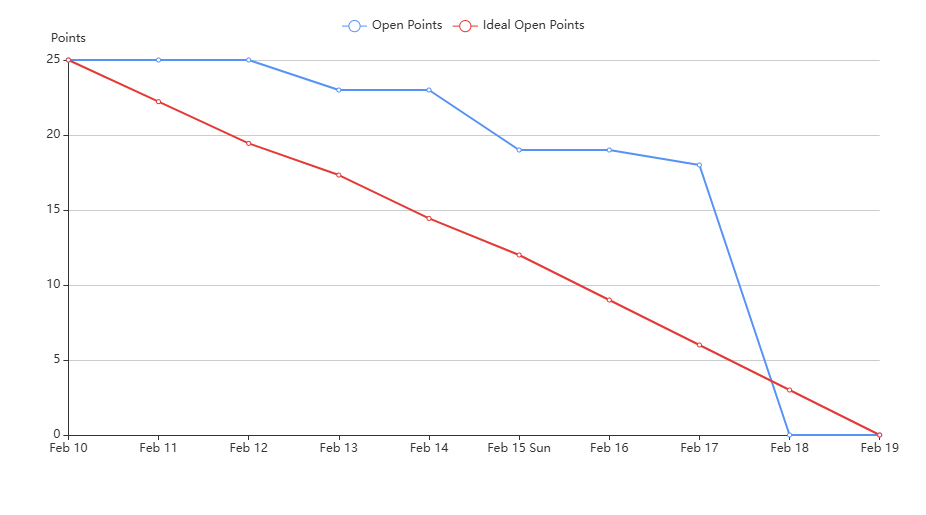
\includegraphics[width=0.7\linewidth, keepaspectratio]{img/BR_Sprint8}
	\caption[Burndown Report del Sprint 8]{Burndown Report del Sprint 8.}
	\label{fig:brsprint8}
\end{figure}

Como se observa en el \textit{burndown} (Figura~\ref{fig:brsprint8}), la reducción de \textit{open points} fue más lenta que la ideal durante la mayor parte del \textit{sprint}, debido a los ajustes iterativos en la interfaz y la infraestructura, tareas que ocupaban un gran número de puntos, aunque fueron siendo ejecutadas durante toda la semana; no obstante, en los últimos días se cerró un bloque grande de trabajo, quedando el \textit{sprint} prácticamente completado el 18 de febrero, un día antes de lo planificado.

\subsection{Sprint 9 - Cierre de la release}
Este \textit{sprint} abarcó del 19 al 26 de febrero, con una duración de una semana. La planificación inicial contemplaba 22~horas de trabajo, a las que se sumaban 2~\textit{points} de una tarea erróneamente realizada del \textit{sprint} anterior, por lo que la carga prevista equivalía aproximadamente a 24~horas. Finalmente, la dedicación real fue de 25~horas y 25~minutos.

Los objetivos definidos para este \textit{sprint} fueron los siguientes:
\begin{itemize}
	\item Volver a ajustar el diagrama de casos de uso.
	\item Finalizar la lógica de Babel y completar la traducción de la aplicación.
	\item Añadir referencias a imágenes y corregir varios detalles del Capítulo 6, \textit{Trabajos relacionados}.
	\item Redactar la comparativa entre los modelos basados en \textit{pickle} y PyTorch.
	\item Corregir distintos aspectos del código y de la interfaz de la aplicación:
	\begin{itemize}
		\item Eliminar la duplicidad existente en la ruta \texttt{calculate}.
		\item Extraer el \textit{script} embebido en \texttt{index.html} a un fichero \texttt{.js} independiente.
		\item Crear un hipervínculo al sitio web de la UBU en el \textit{footer}.
		\item Eliminar el botón específico de trazas.
		\item Sustituir las alertas previas por notificaciones flotantes tipo \textit{toast}.
		\item Crear e insertar un logotipo para la web (\textit{favicon}).
		\item Corregir el comportamiento visual del campo \textit{choose file}.
	\end{itemize}
	\item Sustituir la lógica de inferencia basada en PyTorch por una nueva lógica adaptada a los modelos en \textit{pickle}.
	\item Implementar la descarga de la imagen original, la imagen resultante y el JSON de trazas.
	\item Crear una tabla descriptiva de \textit{encoders} y corregir varios aspectos del Capítulo 3, \textit{Conceptos teóricos}.
	\item Completar la redacción de \textit{sprints} anteriores que todavía tenía pendientes.
\end{itemize}

En primer lugar, volví a ajustar el diagrama de casos de uso, ya que todavía no estaba completamente cerrado a nivel visual. Para ello, reorganicé la disposición de la mayor parte de los casos de uso y afiné su colocación para que el resultado fuese más claro y equilibrado desde el punto de vista gráfico.

A continuación, terminé la lógica de traducción mediante Flask-Babel. Como en el \textit{sprint} anterior me había limitado a dejar preparada la infraestructura, en este ya encapsulé todos los textos necesarios y completé su traducción a los otros cuatro idiomas disponibles: inglés, francés, italiano y alemán, utilizando los correspondientes ficheros \texttt{.po}. Esta parte la desarrollé en dos días distintos, dejando así cerrada la base de internacionalización de la aplicación.

Después, ajusté algunos elementos del apartado de \textit{Trabajos relacionados} que todavía no estaban del todo pulidos y redacté la comparativa entre los modelos en \textit{pickle} y en PyTorch a partir de los resultados obtenidos en el \textit{notebook} de pruebas del \textit{sprint} anterior. Con ello, dejé documentada la justificación técnica del cambio de enfoque en la inferencia.

Posteriormente, abordé varios cambios en el código y en la interfaz de la web. En esta fase eliminé la duplicidad de la ruta \texttt{calculate}, separé el código JavaScript que se encontraba embebido en \texttt{index.html} para pasarlo a un fichero \texttt{.js} independiente y dejé la estructura del \textit{frontend} algo más limpia y mantenible. También añadí un hipervínculo al sitio web de la UBU en el \textit{footer}, eliminé el botón específico de visualización del \texttt{.json} de trazas al no resultar ya necesario dentro del flujo definitivo, sustituí las alertas previas por notificaciones flotantes tipo \textit{toast}, incorporé un \textit{favicon} propio para dar una identidad visual más cuidada a la aplicación y corregí el comportamiento del campo de selección de archivos, que visualmente no estaba mostrando un resultado adecuado y no se podía traducir correctamente con  Flask-Babel.

Más adelante, llevé a cabo la tarea central del \textit{sprint}, que fue sustituir toda la lógica de inferencia que había preparado para PyTorch por una nueva lógica adaptada a los modelos serializados mediante \textit{pickle}. Esta transición me ocupó un par de días, ya que requería reajustar el flujo de carga y ejecución para que el comportamiento en la aplicación quedase alineado con la decisión técnica tomada tras la comparativa previa.

Además, implementé la lógica de descarga tanto de la imagen original como de la imagen resultante y del JSON de trazas, con el objetivo de que el usuario pudiese conservar fácilmente los archivos generados durante el procesamiento. Con ello, la aplicación resultó más completa desde el punto de vista funcional y más cercana al cierre de la primera \textit{release}.

Por último, realicé varias correcciones en el Capítulo 3 del documento de la memoria, destacando especialmente la creación de una tabla para presentar de forma estructurada los \textit{encoders} empleados en el artículo científico en el que baso el proyecto~\cite{diezpastora2025trails}. Paralelamente, aproveché este \textit{sprint} para terminar de redactar los \textit{sprints} anteriores que seguían pendientes desde hacía varias iteraciones, dejando así la planificación temporal mucho más alineada con el estado real del trabajo.

\begin{figure}
	\centering
	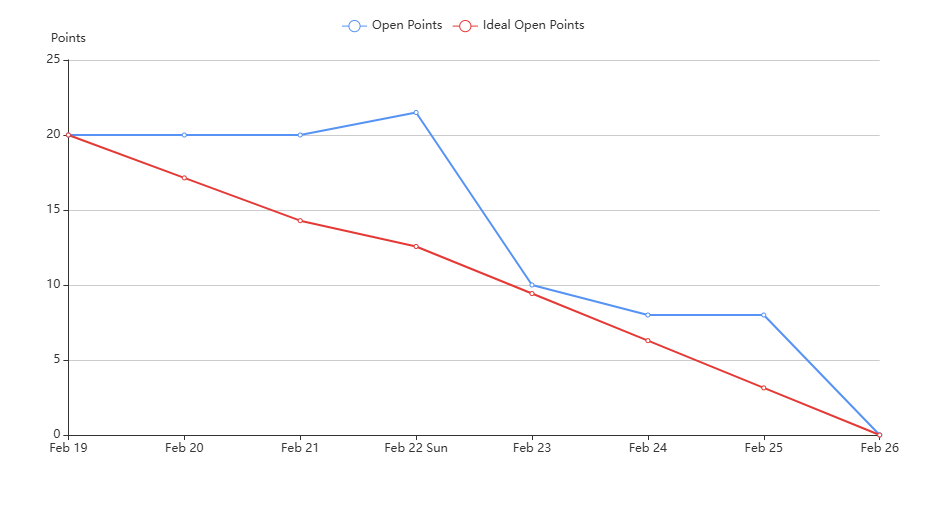
\includegraphics[width=0.7\linewidth]{img/BR_Sprint9}
	\caption[Burndown Report del Sprint 9]{Burndown Report del Sprint 9.}
	\label{fig:brsprint9}
\end{figure}

Como se observa en el burndown de este \textit{sprint} (Figura~\ref{fig:brsprint9}), durante los primeros días el avance fue más lento e incluso hubo un ligero repunte de \textit{open points}, debido a que seguían apareciendo ajustes derivados del cierre técnico de la \textit{release}. No obstante, a partir de la resolución de las tareas principales de integración y refactorización, el volumen pendiente descendió con rapidez, quedando el \textit{sprint} completamente cerrado el 26 de febrero, cerrando así la primera \textit{release} ese mismo día tras la reunión semanal.

\subsection{Sprint 10 - Primeros pasos con Google Earth Engine}
El \textit{Sprint 10} se centró en abrir una nueva línea de trabajo orientada a la integración de Google Earth Engine (GEE) como alternativa para la obtención de imágenes de entrada, a la vez que se consolidaban pequeños ajustes en la aplicación web y en la documentación. Este \textit{sprint} abarcó del 26/02/26 hasta el 05/03/26 y estimé una dedicación total de 25~horas, aunque finalmente invertí 21,4~horas, al poder cerrar varias tareas con menor esfuerzo del previsto.

Los objetivos definidos para este \textit{sprint} fueron los siguientes:
\begin{itemize}
	\item Aplicar cambios puntuales en la aplicación web:
	\begin{itemize}
		\item Renombrar el \textit{checkbox} para mostrarlo como: Dibujar trazas.
		\item Permitir que un clic sobre \textit{upload image} activase también la selección de archivo.
	\end{itemize}
	\item Generar el listado de dependencias mediante \texttt{pip freeze}.
	\item Eliminar el reescalado de imagen en una prueba concreta para verificar correctamente el dibujado de trazas.
	\item Corregir algunos puntos de la memoria y anexos:
	\begin{itemize}
		\item Ajustar el formato de listados asociados a métricas como TP, FP, FN, etc.
		\item Explicar la incidencia e interpretación de los gráficos \textit{burndown} en el apartado A de anexos.
	\end{itemize}
	\item Configurar extensiones y convenciones PEP8 y reforzar la documentación del código.
	\item Arreglar y consolidar \textit{tests} de flujo.
	\item Iniciar las primeras implementaciones con Google Earth Engine:
	\begin{itemize}
		\item Investigar licencias y límites asociados a la nueva implementación.
		\item Crear un \textit{notebook} base de GEE (autenticación, consulta inicial y \textit{preview}).
		\item Preparar un \textit{notebook} para descarga de imágenes mediante colecciones de GEE.
		\item Construir un prototipo HTML mínimo para seleccionar un área mediante dos clics y descargar imágenes del rectángulo definido para su posterior segmentación.
	\end{itemize}
\end{itemize}

En primer lugar, realicé varios ajustes pequeños pero necesarios en la aplicación web para mejorar la claridad del flujo de uso. En concreto, renombré el \textit{checkbox} asociado a la visualización para que apareciese como Dibujar trazas, alineándolo con la lógica del momento de la interfaz, y adapté el comportamiento del botón de \textit{upload image} para que un clic sobre el propio elemento activase también la selección del archivo, haciendo la interacción más directa.

A continuación, consolidé el entorno de desarrollo y documentación del proyecto. Por un lado, generé el listado de dependencias mediante \texttt{pip freeze} para dejar registradas las versiones exactas del entorno. Por otro, configuré extensiones de estilo PEP8 y reforcé la documentación del código, de forma que la base quedase más mantenible y homogénea. En paralelo, realicé una prueba concreta eliminando el reescalado de la imagen, ya que necesitaba verificar el flujo del funcionamiento del dibujado de trazas. Tras esto, logré conseguir una versión correcta del mismo.

También dediqué parte del \textit{sprint} a corregir detalles en la memoria y anexos.

Hacia el final del \textit{sprint} incorporé una tarea no prevista inicialmente: arreglar y consolidar \textit{tests} de flujo. Esta necesidad surgió el martes 03/03/26, a dos días del cierre del \textit{sprint}, y me sirvió para asegurar que los cambios recientes no rompían el comportamiento esperado en el circuito principal de uso.

Por último, el bloque más relevante del \textit{sprint} fue el inicio de las primeras implementaciones con Google Earth Engine. Comencé investigando licencias y límites de uso para entender las restricciones reales del servicio. Aquí encontré el que probablemente sea el mayor problema del TFG y es que existían limitaciones legales y funcionales para poder llevar a cabo el flujo completo de la aplicación.

A partir de ahí, construí un \textit{notebook} base que resolvía autenticación, una primera consulta y un \textit{preview} de resultados y preparé un segundo, tercer y cuarto \textit{notebook} orientados a la descarga de imágenes mediante colecciones de GEE. 

Más adelante, desarrollé un prototipo HTML mínimo en el que el usuario podía seleccionar un área geográfica mediante dos clics, definiendo así un rectángulo y, a partir de esa selección, descargar imágenes del recuadro para su posterior segmentación. Este avance dejó preparada la base conceptual y técnica para continuar con una integración más completa en los siguientes \textit{sprints}.

\begin{figure}
	\centering
	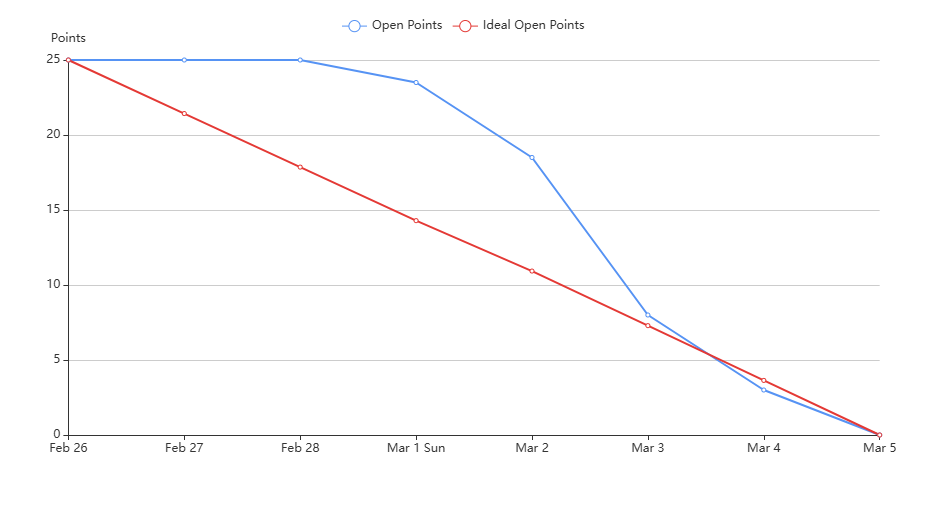
\includegraphics[width=0.7\linewidth]{img/BR_Sprint10}
	\caption[Burndown Report del Sprint 10]{Burndown Report del Sprint 10.}
	\label{fig:brsprint10}
\end{figure}

Como se aprecia en el \textit{burndown} del \textit{sprint} (Figura~\ref{fig:brsprint10}), el volumen de \textit{open points} se mantuvo prácticamente estable durante los primeros días, ya que el trabajo se concentró en investigación y preparación y en tareas de ajuste poco visibles. A partir del 2 de marzo el descenso se aceleró al cerrarse los hitos principales y consolidarse los cambios, quedando el \textit{sprint} completamente finalizado el 5 de marzo.

\subsection{Sprint 11 - Diseños para la nueva funcionalidad}
El \textit{Sprint~11} se desarrolló entre el 5 y el 12 de marzo. Para este \textit{sprint} estimé una dedicación total de 13~horas, y finalmente invertí 12~horas y 35~minutos. En este caso, la planificación ya contemplaba que dispondría de poco tiempo durante la semana, por lo que la mayor parte del trabajo se concentró en los últimos días del \textit{sprint}, avanzando únicamente en tareas clave y de preparación.

Los objetivos definidos para este \textit{sprint} fueron los siguientes:
\begin{itemize}
	\item Corregir el \textit{label} asociado al estado de la imagen en la aplicación.
	\item Mejorar algunos \textit{tests} para que provocasen errores de forma controlada y validasen correctamente el comportamiento esperado.
	\item Crear el \textit{mockup} de las nuevas pantallas necesarias para la siguiente funcionalidad de la aplicación.
	\item Diseñar el modelo de datos: elaborar el diagrama E-R de la aplicación.
\end{itemize}

En primer lugar, realicé un ajuste puntual en la interfaz corrigiendo el \textit{label} que indicaba el estado de la imagen, ya que en algunos casos no reflejaba correctamente la situación del flujo. En paralelo, reforcé ciertos \textit{tests} para que, en escenarios concretos, generasen fallos controlados y permitiesen comprobar que el sistema respondía de forma adecuada ante entradas no válidas o estados inconsistentes.

El bloque principal del \textit{sprint} consistió en preparar el diseño de la nueva funcionalidad. Por un lado, elaboré el \textit{mockup} de las pantallas adicionales para fijar el flujo de interacción y clarificar qué elementos debían incorporarse en la aplicación. Por otro, trabajé en el diseño de base de datos: mi intención era construir el diagrama entidad--relación (E-R), pero terminé generando directamente el esquema relacional. Posteriormente detecté que esta aproximación no era la correcta para el entregable esperado, por lo que dejé previsto corregirlo y completar el diagrama en el \textit{sprint} siguiente.

Finalmente, al cierre del \textit{sprint}, subí al repositorio los \textit{notebooks} desarrollados en el \textit{sprint} anterior. No tenía claro si debían incluirse como parte del código versionado o mantenerse únicamente como material de trabajo, y opté por incorporarlos para asegurar trazabilidad, aunque lo hice con una iteración de retraso respecto a cuando se habían elaborado.

\begin{figure}
	\centering
	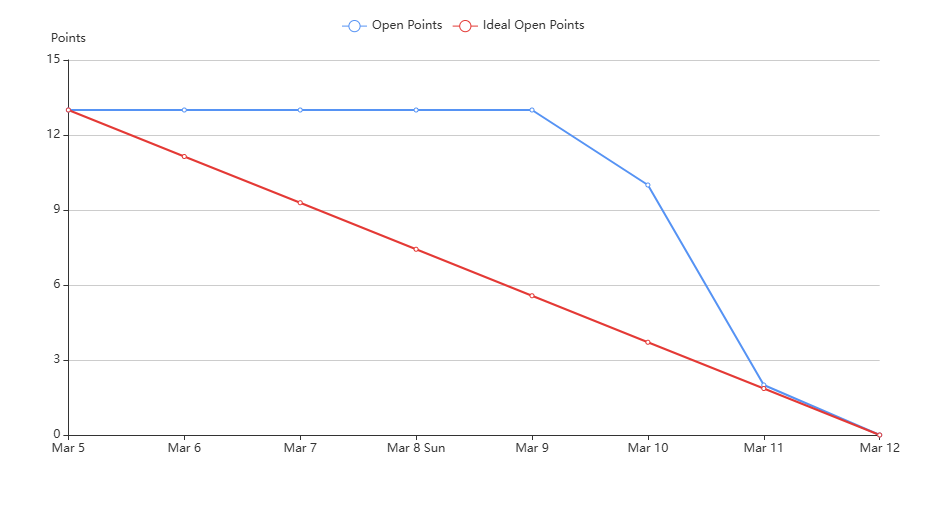
\includegraphics[width=0.7\linewidth]{img/BR_Sprint11}
	\caption[Burndown Report del Sprint 11]{Burndown Report del Sprint 11.}
	\label{fig:brsprint11}
\end{figure}

Como se aprecia en la Figura~\ref{fig:brsprint11}, el avance se mantuvo prácticamente plano durante la mayor parte del \textit{sprint}, concentrándose el cierre de tareas en los últimos días, en línea con la disponibilidad reducida que se había previsto para esta semana.

\subsection{Sprint 12 - Implementación de la funcionalidad geoespacial}
El \textit{Sprint 12} se desarrolló del 12 al 19 de marzo. Para este \textit{sprint} estimé una dedicación total de 17,5~horas y finalmente invertí aproximadamente 18~horas. El objetivo principal de esta iteración fue empezar a materializar la nueva funcionalidad geoespacial en la aplicación, preparando la pantalla referente al visor web y parte de la navegación necesaria para llegar a él.

Los objetivos definidos para este \textit{sprint} fueron los siguientes:
\begin{itemize}
	\item Arreglar el diagrama relacional de la base de datos.
	\item Crear el diagrama entidad--relación (E-R) de la BBDD.
	\item Investigar el alcance del PNOA y su adecuación como fuente de datos.
	\item Crear un menú de navegación en la \textit{navbar}.
	\item Adaptar el prototipo inicial al visor web.
	\item Arreglar el apéndice B de los anexos.
	\item (Pendiente) Crear dos pantallas nuevas asociadas a la funcionalidad geoespacial: colección y galería de imágenes.
\end{itemize}

Durante los primeros días me centré en consolidar la estructura de la base de datos, ya que era imprescindible para que la nueva funcionalidad quedase bien definida. En primer lugar, corregí el esquema relacional que había generado en el \textit{sprint} anterior, y a continuación elaboré el diagrama E-R de la aplicación, de manera que el diseño quedase documentado de forma correcta y consistente antes de seguir ampliando la implementación.

En paralelo, dediqué tiempo a investigar el alcance del PNOA, revisando qué cobertura ofrecía y en qué condiciones podía utilizarse dentro del flujo previsto para el proyecto. Esta parte fue relevante para validar que la fuente de datos era viable y para acotar el tipo de consultas y descargas que podrían integrarse más adelante.

En cuanto a la aplicación, implementé un menú en la \textit{navbar} para preparar la navegación entre pantallas, y adapté el prototipo previo para que encajase con el visor web, dejando un flujo mínimo funcional y alineado con el enfoque geoespacial. Sin embargo, aunque dentro de la planificación se contemplaban también dos pantallas adicionales, que suponían aproximadamente 8~horas de trabajo y ya estaban contabilizadas dentro de las horas estimadas, no llegué a completarlas en este \textit{sprint}. La mayor parte del esfuerzo se concentró en estabilizar la base y en dejar el visor preparado, posponiendo esas pantallas para la siguiente iteración.

Además, el lunes 16 surgió una tarea no prevista inicialmente: corregir el apéndice B de los anexos. La cerré ese mismo día, aprovechando que se trataba de un ajuste acotado y necesario para mantener la coherencia del documento.

\begin{figure}
	\centering
	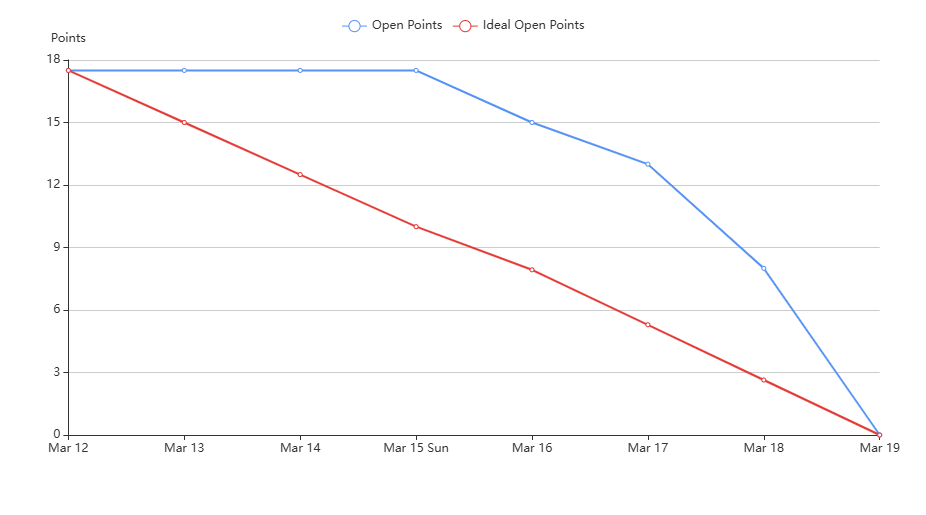
\includegraphics[width=0.7\linewidth]{img/BR_Sprint12}
	\caption[Burndown Report del Sprint 12]{Burndown Report del Sprint 12.}
	\label{fig:brsprint12}
\end{figure}

Como se aprecia en la Figura~\ref{fig:brsprint12}, el \textit{burndown} se mantiene prácticamente plano durante los primeros días, reflejando que gran parte del trabajo estuvo orientado a preparación e investigación y a tareas que no cerraban \textit{points} de forma inmediata. A partir de la mitad del \textit{sprint} el descenso se vuelve más pronunciado, coincidiendo con el cierre progresivo de tareas técnicas y con la incorporación y resolución de la incidencia del apéndice B. Finalmente, el \textit{sprint} se completa el 19 de marzo, quedando únicamente como arrastre la creación de las pantallas de colección y galería, previstas pero no finalizadas.

\subsection{Sprint 13 - Colecciones de imágenes}
El \textit{Sprint 13} se desarrolló del 20 al 26 de marzo. Para este \textit{sprint} estimé una dedicación de 19~horas, y finalmente invertí 20~horas y 35~minutos. El objetivo principal de esta iteración fue completar la funcionalidad asociada a la gestión de colecciones y galerías de imágenes, cerrando además ajustes pendientes en la documentación y realizando una nueva validación del flujo de descarga con PNOA.

Los objetivos definidos para este \textit{sprint} fueron los siguientes:
\begin{itemize}
	\item Arreglar la bibliografía de anexos.
	\item Corregir y consolidar los diagramas E-R y relacional:
	\begin{itemize}
		\item Eliminar claves foráneas del diagrama E-R para mantenerlo en un nivel de abstracción correcto.
		\item Ajustar la longitud de ciertos campos.
		\item Añadir un nuevo campo booleano para indicar si una imagen tiene las trazas calculadas o no.
	\end{itemize}
	\item Arreglar el \textit{checkbox} e incorporar la funcionalidad nueva asociada.
	\item Actualizar los \textit{mockups} para incorporar cambios derivados de la nueva funcionalidad:
	\begin{itemize}
		\item Añadir un indicador por imagen en la galería para mostrar si ya tiene las trazas calculadas.
		\item Incluir, en la visualización ampliada, opciones para dibujar y calcular trazas.
		\item Reflejar el estado de cada colección, apoyándolo en consultas a base de datos.
		\item Incorporar opciones de eliminación de elementos en la colección.
		\item Permitir la descarga de un \texttt{.zip} desde la colección.
	\end{itemize}
	\item Ajustar el formato de las imágenes a apaisado, manteniendo la relación 1024$\times$640.
	\item Realizar pruebas con PNOA:
	\begin{itemize}
		\item Cambiar el nombre del \textit{manifest} a \texttt{log.json}.
		\item Probar de nuevo la descarga y verificar el fallo de conexión por \textit{time limit}.
	\end{itemize}
	\item Revisar y ajustar el material gráfico de la memoria:
	\begin{itemize}
		\item Exportar diagramas a PDF.
		\item Actualizar el \textit{mockup} para incluir todas las páginas y redactar una breve explicación para cada una.
	\end{itemize}
	\item Crear las pantallas correspondientes a la nueva funcionalidad de colección y galería de imágenes.
\end{itemize}

En primer lugar, realicé ajustes, centrados en corregir la bibliografía correspondiente a los anexos. En paralelo, consolidé el diseño de base de datos: revisé tanto el diagrama E-R como el relacional, eliminando del E-R las claves foráneas para que quedase correctamente expresado a nivel conceptual, ajustando la longitud de algunos campos de texto y añadiendo un nuevo atributo booleano en la tabla de imágenes para reflejar de manera directa si las trazas estaban calculadas o no.

A continuación, corregí el \textit{checkbox} de la aplicación para aportarle una nueva funcionalidad. Actualicé también los \textit{mockups}, incorporando indicadores de estado por imagen, opciones en la vista ampliada para dibujar y calcular, y el estado general de cada colección. Además, añadí acciones complementarias, siendo estas la eliminación de elementos dentro de una colección y la descarga de un \texttt{.zip} directamente desde esa pantalla.

En el apartado visual, ajusté el formato de las imágenes, obtenidas mediante el mapa, a apaisado manteniendo la relación 1024$\times$640, de forma que se pudiese acercar más a aquellas que se usaron para entrenar el modelo. También actualicé el material gráfico de la memoria: exporté diagramas a PDF y reorganicé el \textit{mockup} para incluir todas las páginas, añadiendo una descripción para todas y cada una de ellas.

Por otro lado, realicé ciertas pruebas de conexión con PNOA y cambié el nombre del \textit{manifest} a \texttt{log.json}.

Finalmente, el bloque central del \textit{sprint} consistió en crear las diferentes pantallas asociadas a la funcionalidad: la pantalla de colección y la galería de imágenes. Para llevar esto a cabo, tuve que definir también la base de datos con SQLite, como he comentado antes y preparar un lanzado automático de la misma.

\begin{figure}
	\centering
	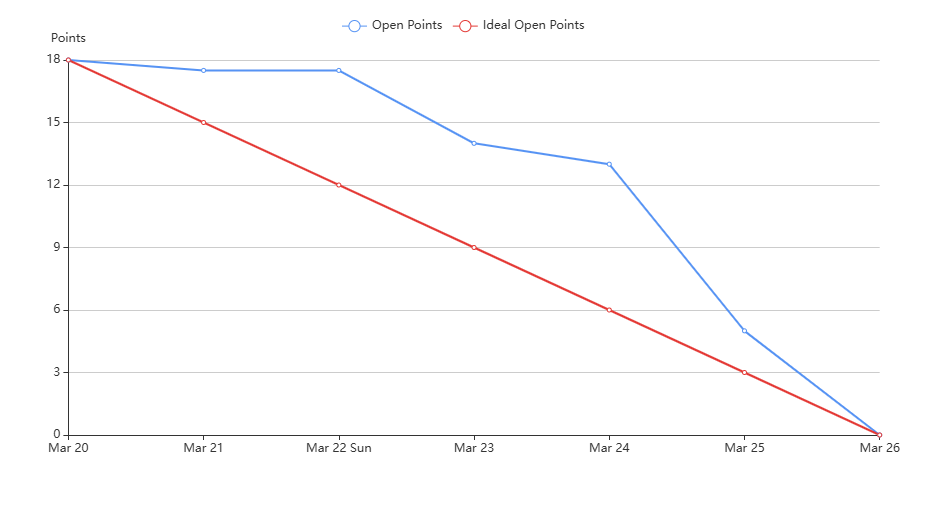
\includegraphics[width=0.7\linewidth]{img/BR_Sprint13}
	\caption[Burndown Report del Sprint 13]{Burndown Report del Sprint 13.}
	\label{fig:brsprint13}
\end{figure}

Como muestra la Figura~\ref{fig:brsprint13}, el avance se mantuvo relativamente estable durante los primeros días, al concentrarse el trabajo en ajustes de diseño y en tareas de preparación. A partir del 23--24 de marzo el descenso se acelera, coincidiendo con el cierre de las pantallas principales y la consolidación de la nueva lógica de estado en la interfaz, quedando el \textit{sprint} cerrado el 26 de marzo.

\subsection{Sprint 14 - Ajustes y consolidación durante Semana Santa}
El \textit{Sprint 14} se desarrolló durante el periodo de Semana Santa. Para esta iteración estimé una dedicación total de 26~horas, y finalmente invertí 24~horas y 25~minutos. En esta iteración el avance estuvo condicionado por carga académica: durante los primeros días apenas pude progresar y, además, el \textit{sprint} se amplió un día adicional. A partir de ese punto, el grueso del trabajo se concentró en la segunda mitad del \textit{sprint}, donde fui cerrando tareas de forma progresiva hasta completar el bloque planificado.

Los objetivos definidos para este \textit{sprint} fueron los siguientes:
\begin{itemize}
	\item Modificar el apartado de métricas en la memoria.
	\item Ajustar el \textit{layout} del mapa.
	\item Modificar la lógica de imágenes para mantener la relación de aspecto.
	\item Incorporar \textit{tooltips} en el visor.
	\item Añadir un campo de descripción para cada zona.
	\item Cambiar la previsualización de imagen por la previsualización de la zona seleccionada.
	\item Implementar la lógica de trazas en segundo plano.
	\item Redactar una explicación del problema de licencias asociado a GEE.
	\item Corregir aspectos relevantes de la memoria.
	\item Implementar la lógica de visualización de imagen en grande.
	\item Investigar posibles errores en el mapa.
	\item Investigar posibles errores en la colección de imágenes.
\end{itemize}

Durante los primeros días prioricé ajustes de documentación y cambios que no requerían una implementación extensa. En concreto, revisé el apartado de métricas de la memoria para mejorar su claridad, y realicé correcciones puntuales en secciones relevantes del documento, con el objetivo de mantener el texto alineado con la evolución real de la aplicación.

A continuación, centré el trabajo en consolidar el flujo del visor geoespacial. Por un lado, ajusté el \textit{layout} del mapa e incorporé \textit{tooltips} para mejorar la interpretabilidad de la interfaz. Por otro, modifiqué la lógica de imágenes para conservar correctamente la relación de aspecto, para que así las imágenes se parecieran más a las de entrenamiento. Hice también que se pudiera cambiar el nombre de cada galería y cambié la previsualización para que, en lugar de mostrar únicamente la primera imagen, se mostrase la \textit{preview} de la zona seleccionada completa.

En la parte más técnica del \textit{sprint}, creé la lógica de trazas en segundo plano y la visualización de la imagen en grande, de forma que la aplicación pudiese gestionar mejor operaciones de cálculo sin bloquear la experiencia de uso y, al mismo tiempo, permitir una inspección más cómoda del resultado. Además, documenté de forma específica el problema de licencias asociado a GEE, ya que era necesario dejar constancia en la memoria de las limitaciones y condicionantes de uso de esta tecnología.

Por último, reservé parte del cierre del \textit{sprint} a tareas de verificación: investigué posibles errores tanto en el mapa como en la colección de imágenes, revisando el comportamiento en casos límite y buscando incoherencias derivadas de los cambios recientes.

\begin{figure}
	\centering
	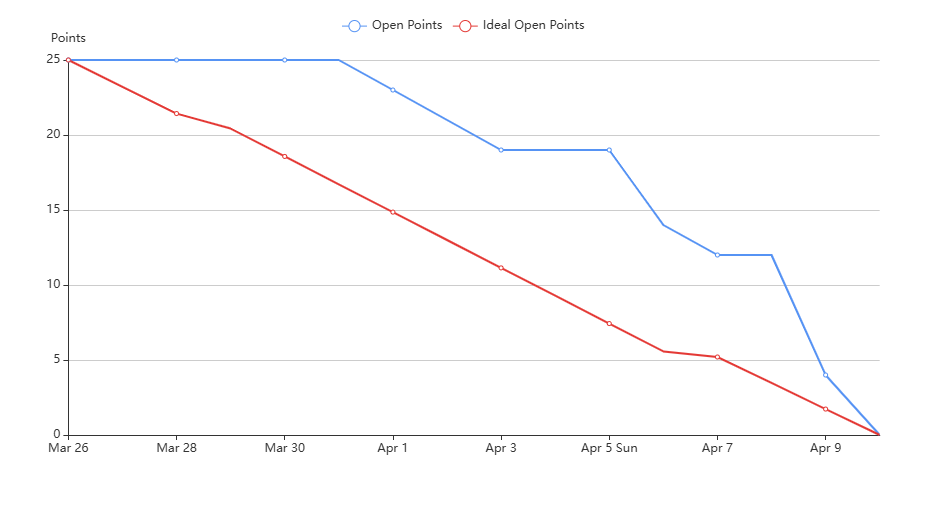
\includegraphics[width=0.7\linewidth]{img/BR_Sprint14}
	\caption[Burndown Report del Sprint 14]{Burndown Report del Sprint 14.}
	\label{fig:brsprint14}
\end{figure}

Como se aprecia en la Figura~\ref{fig:brsprint14}, el \textit{burndown} refleja un inicio prácticamente plano, coherente con la menor disponibilidad de los primeros días. También se observa un ajuste en la línea ideal, debido a la ampliación del \textit{sprint} en un día por motivos académicos. A partir de la mitad del periodo el descenso se acelera, mostrando cómo el cierre de tareas se concentró en los últimos días, hasta completar el \textit{sprint} al final de la semana.

\subsection{Sprint 15 - Integración de usuarios y administración}
El \textit{Sprint 15} se extendió durante casi dos semanas. Aunque inicialmente estaba planificado como un \textit{sprint} de una semana, por diversos motivos se decidió aplazar el cierre una semana adicional en el último momento, lo que afectó directamente a la planificación y explica que el \textit{burndown report} presente un comportamiento menos lineal de lo habitual. 

Para este \textit{sprint} estimé una dedicación total de 23~horas y finalmente invertí 25~horas y 30~minutos. Durante los primeros días apenas pude avanzar y, además, una parte importante del trabajo consistió en tareas estructurales que requerían acumular varios cambios antes de poder dar cierres completos, por lo que el progreso quedó más concentrado al final del periodo.

Los objetivos definidos para este \textit{sprint} fueron los siguientes:
\begin{itemize}
	\item Ajustar la interfaz del visor:
	\begin{itemize}
		\item Cambiar el ancho del mapa para que ocupase toda la pantalla.
		\item Añadir un \textit{checkbox} de ``trazas dibujadas'' en cada tesela.
		\item Modificar la \textit{preview} de la zona seleccionada para que se almacenase directamente en memoria.
	\end{itemize}
	\item Optimizar la lógica del \textit{worker} para evitar comprobaciones continuas innecesarias.
	\item Diseñar el \textit{mockup} completo de la funcionalidad de usuarios.
	\item Reestructurar la interacción con la base de datos, pasando de inserciones manuales a SQLAlchemy.
	\item Implementar el sistema de usuarios:
	\begin{itemize}
		\item Crear pantallas de \textit{login} y registro.
		\item Crear un menú de administrador.
		\item Definir permisos de acceso a pantallas en función del tipo de usuario.
		\item Crear un panel de gestión de usuarios.
		\item Crear un panel de gestión del modelo.
	\end{itemize}
\end{itemize}

En los primeros días abordé cambios principalmente visuales y de comportamiento del visor. En primer lugar, ajusté el mapa para que ocupase todo el ancho disponible, mejorando la experiencia de navegación y evitando el desaprovechamiento de espacio en pantallas grandes. A continuación, añadí un indicador por tesela mediante un \textit{checkbox} asociado a si las trazas estaban dibujadas, lo que facilitaba distinguir rápidamente el estado de cada elemento dentro de la vista. En paralelo, modifiqué la lógica de \textit{preview} de la zona seleccionada para que se almacenase directamente en memoria, reduciendo dependencias con almacenamiento temporal y simplificando el flujo de consulta y representación asociados a esta funcionalidad.

Seguidamente, realicé ajustes internos para mejorar robustez. En concreto, modifiqué la lógica del \textit{worker} para que no estuviese comprobando continuamente el estado de forma activa, sino que operase de manera más eficiente.

La segunda mitad del \textit{sprint} se centró en la nueva funcionalidad de usuarios. Primero elaboré el \textit{mockup} completo para tener claro el flujo de pantallas y el rol de cada perfil. A partir de ahí, reestructuré la interacción con base de datos: sustituí inserciones manuales por un enfoque basado en SQLAlchemy, de forma que el acceso a datos quedase más mantenible y coherente con el crecimiento del proyecto. Una vez estabilizada esta base, implementé las pantallas de \textit{login} y registro y construí el menú de administrador.

Finalmente, desarrollé la capa de permisos, restringiendo el acceso a determinadas pantallas en función del tipo de usuario y del rol asignado, y creé los paneles de administración: uno para la gestión de usuarios y otro orientado a la gestión del modelo. Este bloque concentró buena parte del trabajo del \textit{sprint}, ya que dependía de tener cerradas previamente la navegación, la persistencia y la estructura de roles.

\begin{figure}
	\centering
	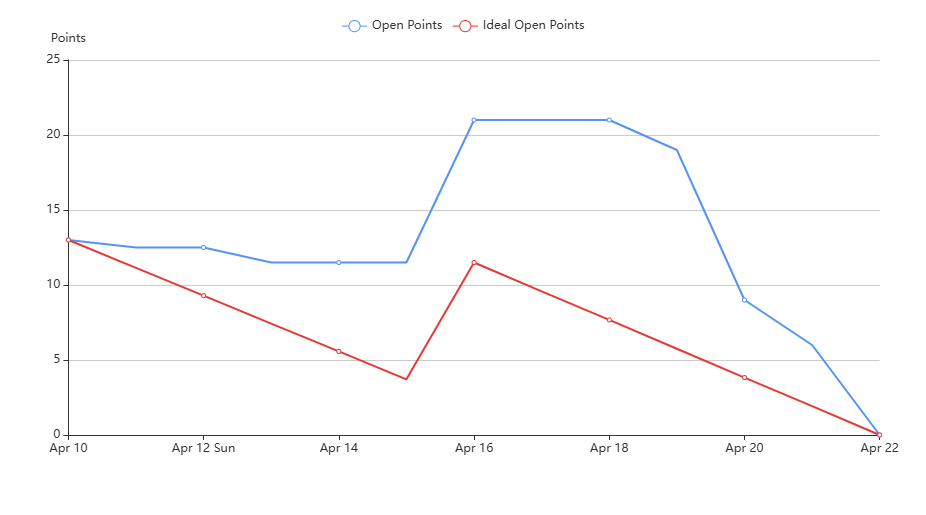
\includegraphics[width=0.7\linewidth]{img/BR_Sprint15}
	\caption[Burndown Report del Sprint 15]{Burndown Report del Sprint 15.}
	\label{fig:brsprint15}
\end{figure}

Como se aprecia en la Figura~\ref{fig:brsprint15}, el \textit{burndown} presenta un comportamiento atípico. Por un lado, el descenso inicial es muy limitado, coherente con la baja disponibilidad de los primeros días y con el hecho de que varias tareas eran estructurales y no se podían cerrar de forma aislada. Por otro, se observa un reajuste a mitad del periodo: en ese punto se amplió el \textit{sprint} una semana adicional y se replanificó la línea ideal, lo que explica el cambio de pendiente en el tramo central. A partir de ahí, el cierre de tareas se concentra al final, cuando ya quedaron consolidadas las dependencias internas y el \textit{sprint} termina con una caída pronunciada hasta completarse el día 22 de abril.

\subsection{Sprint 16 - Cierre de la aplicación}
El \textit{Sprint 16} se desarrolló del 23 al 30 de abril, con una duración de una semana. Para este \textit{sprint} estimé una dedicación total de 22,5~horas, aunque finalmente invertí aproximadamente 25~horas. El foco principal de esta iteración fue consolidar la funcionalidad de usuarios y administración introducida en el \textit{sprint} anterior, mejorar la usabilidad de la interfaz y reforzar la gestión de modelos desde el panel de administrador, poniendo así fin a la funcionalidad principal de la aplicación.

Los objetivos definidos para este \textit{sprint} fueron los siguientes:
\begin{itemize}
	\item Arreglar la página de gestión de usuarios.
	\item Arreglar el desplegable del menú y su comportamiento.
	\item Cambiar el nombre de los \textit{folds} y ajustar la lógica de búsqueda.
	\item Mejorar la gestión de \textit{folds} desde administración:
	\begin{itemize}
		\item Permitir que el administrador renombre \textit{folds}.
		\item Cargar nuevos \textit{folds} y eliminar los existentes.
		\item Validar nuevos modelos por \textit{fold}.
	\end{itemize}
	\item Añadir \textit{tooltips} en las funciones del \textit{home}.
	\item Añadir \textit{tooltips} en la colección y la galería.
	\item Añadir lógica de pintado de trazas en el visor.
	\item Formatear la página de \textit{log in}.
	\item Formatear la página de registro.
	\item Permitir la descarga de informes de usuarios en formato CSV y PDF.
	\item Realizar las traducciones de todas las pantallas.
\end{itemize}

En primer lugar, trabajé en corregir y estabilizar la parte de administración. Ajusté la página de gestión de usuarios, revisando tanto el comportamiento como la presentación, y arreglé el desplegable del menú, ya que en algunos flujos no se mostraban de forma consistente. A partir de ahí, me centré en la gestión del modelo, ya que era una de las piezas críticas del panel de administración: cambié el criterio de nombres y la lógica de búsqueda para que fuese más clara, permití que el administrador renombrase \textit{folds}, añadí la funcionalidad de carga y eliminación de nuevos \textit{folds}, todo ello con un nuevo proceso de validación por detrás.

En paralelo, realicé mejoras de usabilidad en la interfaz. Añadí \textit{tooltips} en todas las pantalla que faltaban de emplear estos servicios, con el objetivo de guiar al usuario y reducir ambigüedades en acciones frecuentes. Además, implementé la lógica de pintado de trazas directamente en el visor, para así finalizar el flujo del sistema.

También dediqué parte del \textit{sprint} a mejorar la apariencia de las pantallas de autenticación, formateando tanto la página de \textit{log in} como la de registro para que siguiesen el mismo estilo visual del resto de la aplicación. Como cierre de funcionalidad en el área de administración, añadí la posibilidad de descargar información de usuarios en formato CSV y PDF, facilitando la exportación de datos desde el panel.

Por último, completé la traducción de todas las pantallas, integrando los textos en el flujo de internacionalización para que la aplicación quedase consistente en los cinco disponibles.

Cabe señalar que, en los últimos días del \textit{sprint}, se incorporaron dos tareas adicionales: exportación CSV/PDF y traducción completa de pantallas. Como consecuencia, tuve que prescindir de una tarea inicialmente prevista: cargar usuarios automáticamente al lanzar Flask, que quedó fuera del alcance de esta iteración para priorizar los cambios añadidos.

También, recalcar que, tras finalizar este sprint, lancé la segunda release de la aplicación, la 0.8, esto debido a que ya había logrado un buen flujo del sistema.

\begin{figure}
	\centering
	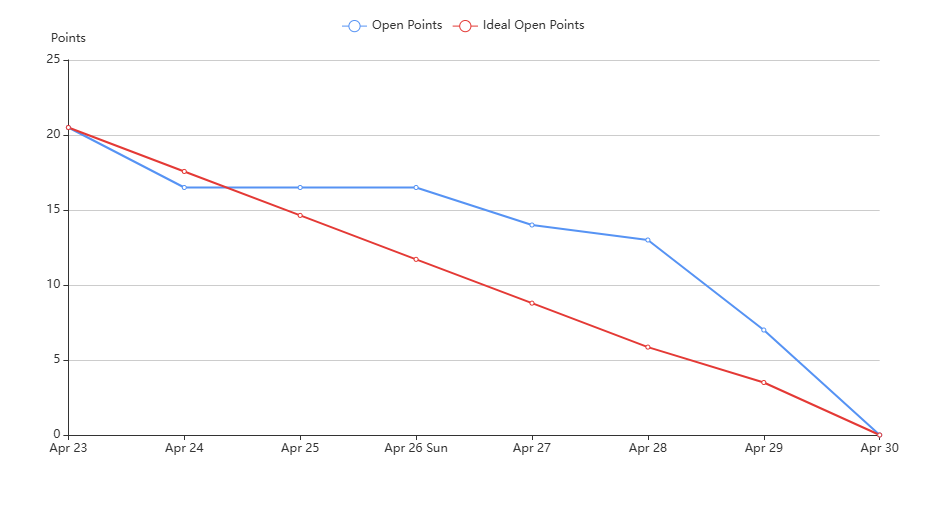
\includegraphics[width=0.7\linewidth]{img/BR_Sprint16}
	\caption[Burndown Report del Sprint 16]{Burndown Report del Sprint 16.}
	\label{fig:brsprint16}
\end{figure}

Como muestra la Figura~\ref{fig:brsprint16}, el \textit{burndown} refleja un descenso progresivo y estable durante la semana, con una ligera pérdida de alineación respecto a la línea ideal en el tramo final. Esto se debe a la incorporación de tareas en los últimos días, lo que incrementó la carga restante cuando el \textit{sprint} ya estaba avanzado. Aun así, el cierre se completó el 30 de abril, consolidando el bloque final de la aplicación.

\subsection{Sprint 17 - Arreglos funcionales y avances en la memoria}
El \textit{Sprint 17} se desarrolló del 1 al 7 de mayo, con una duración de una semana. Para este \textit{sprint} estimé una dedicación inicial de 20~horas, aunque finalmente invertí aproximadamente 24~horas. Fue una iteración especialmente problemática, ya que gran parte del tiempo se destinó a modificar y depurar la BBDD, lo que bloqueó varias tareas que dependían directamente de ella y provocó que no pudiera cerrar tanto trabajo como estaba previsto.

Los objetivos definidos para este \textit{sprint} fueron los siguientes:
\begin{itemize}
	\item Realizar primeras comprobaciones con \texttt{pytest-cov}.
	\item Cambiar nombres confusos de la interfaz.
	\item Establecer los requisitos funcionales y no funcionales.
	\item Cambiar y actualizar la parte de Google Earth Engine (GEE) en la memoria.
	\item Incorporar funcionalidad de fotos para los usuarios.
	\item Redactar el apartado de técnicas y herramientas.
	\item Corregir un \textit{bug} relacionado con las imágenes en la gestión de usuarios.
	\item Cargar usuarios cuando se lance Flask y revisar toda la BBDD.
	\item Permitir eliminar un usuario y sus parcelas en cascada.
	\item Hacer el servicio de \textit{folds} en segundo plano y admitir cualquier nombre para los modelos.
	\item Redactar el manual del programador.
\end{itemize}

Durante los primeros días realicé algunos avances funcionales y de documentación. Por un lado, cambié nombres confusos de la interfaz para que las acciones fuesen más claras para el usuario y empecé a revisar la integración de \texttt{pytest-cov}, aunque esta parte no quedó consolidada hasta el \textit{sprint} siguiente. Por otro lado, establecí los requisitos funcionales y no funcionales del sistema, lo que permitió dejar más claro el alcance real de la aplicación y su comportamiento esperado.

También avancé en la memoria, especialmente en dos frentes. Primero, actualicé la parte relativa a Google Earth Engine, ajustando la redacción para que fuese coherente con los cambios realizados en la funcionalidad geoespacial, ya que ya no usábamos este motor, y con las limitaciones detectadas en \textit{sprints} anteriores. Después, redacté el apartado de técnicas y herramientas, donde se recogían las tecnologías principales utilizadas a lo largo del proyecto y su justificación dentro del desarrollo.

En paralelo, añadí la funcionalidad de fotos para los usuarios y corregí un \textit{bug} relacionado con las imágenes en la página de gestión de usuarios. Aunque este error no era especialmente complejo, sí afectaba a la presentación y coherencia de la interfaz, por lo que era necesario resolverlo antes de seguir ampliando el módulo de administración.

Sin embargo, el mayor problema del \textit{sprint} estuvo en la BBDD. Casi toda la iteración quedó condicionada por cambios y errores derivados de su estructura y de la forma en que interactuaba con las nuevas funcionalidades. Esto me impidió cerrar varias tareas previstas, como cargar usuarios al lanzar Flask, revisar completamente la BBDD, permitir eliminar usuarios junto con sus parcelas en cascada, y hacer que el servicio de \textit{folds} funcionase en segundo plano admitiendo nombres arbitrarios para los modelos. Estas tareas quedaron aplazadas al \textit{sprint} siguiente, donde se resolvería finalmente el bloqueo principal.

Además, quedó pendiente la redacción del manual del programador, ya que requería una revisión más estable del código y de la estructura final de la aplicación. En retrospectiva, durante este \textit{sprint} fui resolviendo distintos flujos de error asociados a la BBDD, pero no los desglosé en tarjetas independientes, por lo que parte del esfuerzo realizado no quedó reflejado con tanta precisión en el tablero.

\begin{figure}
	\centering
	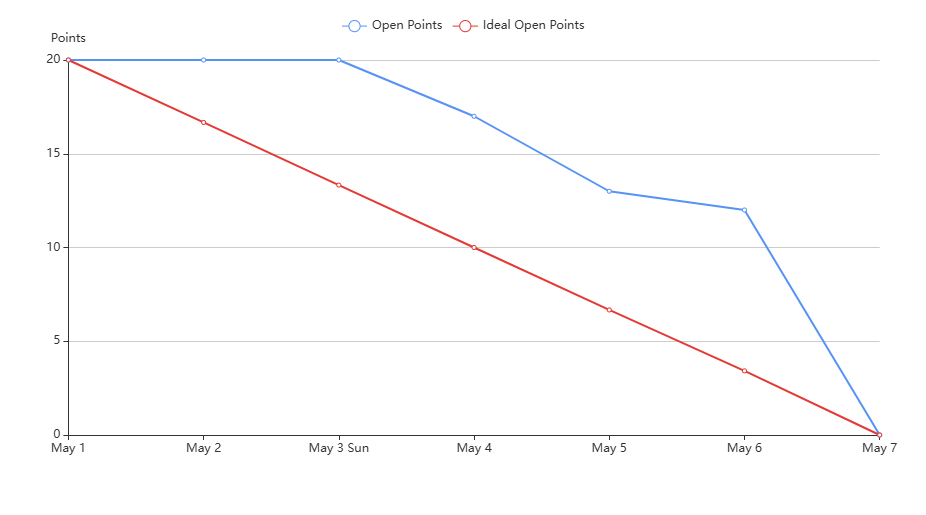
\includegraphics[width=0.7\linewidth]{img/BR_Sprint17}
	\caption[Burndown Report del Sprint 17]{Burndown Report del Sprint 17.}
	\label{fig:brsprint17}
\end{figure}

Como se observa en la Figura~\ref{fig:brsprint17}, el \textit{burndown} muestra un avance irregular. La línea de \textit{open points} desciende poco durante buena parte del \textit{sprint}, ya que muchas tareas dependían de resolver primero el problema de la BBDD. La bajada pronunciada del último día no representa tanto un cierre real de todas las tareas, sino principalmente el aplazamiento de varias de ellas al \textit{sprint} siguiente, donde se abordarían una vez desbloqueada la base de datos.

\subsection{Sprint 18 - Definición de arquitecturas y arreglo final de la BBDD}
El \textit{Sprint 18} se desarrolló del 8 al 14 de mayo. Para este \textit{sprint} estimé una dedicación total de 28~horas, y finalmente invertí aproximadamente 32~horas. El foco principal fue dejar estabilizada la base de datos, cerrando problemas que venían bloqueando tareas del \textit{sprint} anterior, y definir de manera clara la arquitectura del sistema, tanto a nivel conceptual como mediante diagramas, además de reforzar la calidad del proyecto con \textit{coverage} y SonarCloud.

Es importante aclarar que las tareas \textit{Cargar usuarios cuando se lance Flask y revisar toda la BBDD}, \textit{Permitir eliminar un usuario y sus parcelas en cascada}, \textit{Hacer el servicio de folds en segundo plano y admitir el nombre que sea para los modelos} y \textit{Primeras comprobaciones con pytest-cov} venían arrastradas del \textit{sprint} anterior. No pude finalizarlas entonces porque, como bien he comentado, existía un problema en la BBDD que impedía avanzar con garantías, y dicho bloqueo quedó resuelto durante este \textit{sprint}, lo que me permitió cerrarlas correctamente.

Los objetivos definidos para este \textit{sprint} fueron los siguientes:
\begin{itemize}
	\item Cargar usuarios cuando se lance Flask y revisar la BBDD (tarea arrastrada).
	\item Implementar el servicio de \textit{folds} en segundo plano y admitir nombres arbitrarios para modelos (tarea arrastrada).
	\item Permitir eliminar un usuario y sus parcelas en cascada (tarea arrastrada).
	\item Primeras comprobaciones con \textit{pytest-cov} (tarea arrastrada).
	\item Cubrir los flecos restantes del \textit{coverage}.
	\item Configurar SonarCloud correctamente.
	\item Redactar el apartado F de anexos (ODS).
	\item Definir y documentar la arquitectura del sistema:
	\begin{itemize}
		\item Crear una arquitectura hexagonal.
		\item Crear el diagrama de arquitectura por capas.
		\item Crear diagramas arquitectónicos adicionales que quedaban pendientes.
		\item Redactar una explicación para este apartado (se pasó al siguiente \textit{sprint}).
	\end{itemize}
	\item Arreglar el diagrama de casos de uso y los diagramas de BBDD.
	\item Redactar aspectos relevantes que todavía faltaban en la memoria.
	\item Corregir un \textit{bug} puntual de la imagen de perfil en la gestión de usuarios.
\end{itemize}

Durante los primeros días el trabajo se centró en desbloquear y consolidar la base de datos, ya que era el requisito previo para poder cerrar varias tareas que estaban pendientes. En esta fase revisé el estado general de la BBDD y dejé implementada la carga de usuarios al iniciar Flask, asegurando que el sistema arrancase con un estado coherente. A partir de ahí, pude retomar la parte de los modelos: implementé el servicio en segundo plano y adapté la lógica para que el sistema aceptase nombres de modelos sin restricciones artificiales. En paralelo, añadí también la eliminación en cascada de un usuario junto con sus parcelas.

A mitad del \textit{sprint} surgió un \textit{bug} menor relacionado con la imagen de perfil en la gestión de usuarios. Aunque no supuso un bloqueo grave, sí era necesario corregirlo para dejar la funcionalidad cerrada y estable, por lo que lo abordé en cuanto apareció.

Una vez estabilizada la base del sistema, el grueso del \textit{sprint} se orientó a la definición de arquitecturas y a la mejora de calidad. Por un lado, trabajé en la parte de documentación técnica, creando la propuesta de arquitectura hexagonal y el diagrama por capas, además de generar otros diagramas arquitectónicos que aportasen una visión adicional al sistema. También revisé y corregí el diagrama de casos de uso y los diagramas asociados a la BBDD para que fuesen consistentes con el estado real del sistema tras los cambios de este tramo.

Por otro lado, reforcé el apartado de calidad del proyecto: configuré SonarCloud correctamente y cerré los flecos restantes de \textit{coverage}, asegurando que el proyecto quedase mejor respaldado por pruebas y con un análisis estático más limpio. Además, redacté el apartado F de anexos relativo a los ODS e incorporé algunos aspectos relevantes que todavía faltaban en la memoria.

Finalmente, aunque la tarea de \textit{Redactar el apartado de arquitecturas} estaba inicialmente planificada para este \textit{sprint}, se complicó más de lo esperado, ya que me llevó varias iteraciones decidir la mejor forma de presentar y justificar la arquitectura y su encaje con el proyecto. Por ello, dejé avanzados los diagramas y el criterio de diseño durante este \textit{sprint}, pero la redacción final del apartado quedó pospuesta y se completaría el primer día del \textit{sprint} siguiente.

\begin{figure}
	\centering
	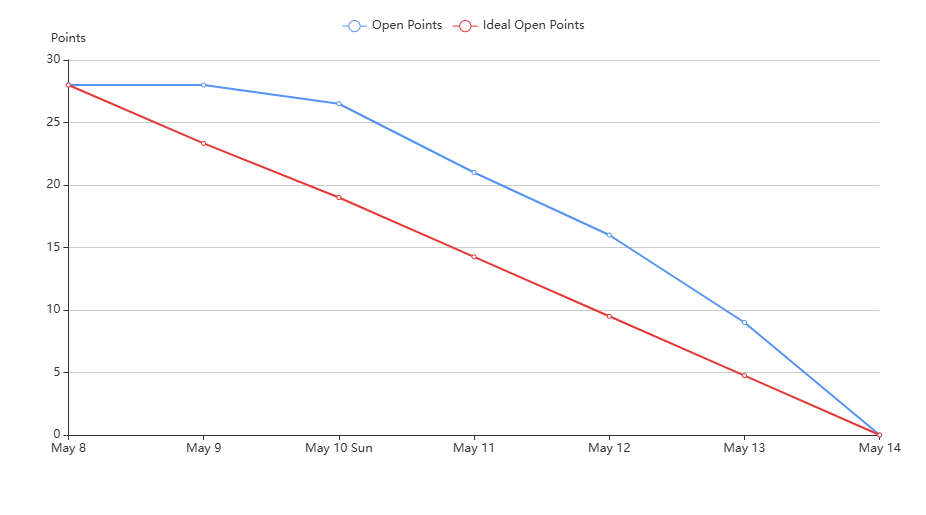
\includegraphics[width=0.7\linewidth]{img/BR_Sprint18}
	\caption[Burndown Report del Sprint 18]{Burndown Report del Sprint 18.}
	\label{fig:brsprint18}
\end{figure}

Como se aprecia en la Figura~\ref{fig:brsprint18}, el \textit{burndown} muestra un inicio prácticamente plano, ya que varias tareas dependían de resolver primero el bloqueo asociado a la BBDD y de consolidar cambios estructurales antes de poder cerrar \textit{issues}. Una vez resueltas esas dependencias, el cierre de tareas se aceleró de forma clara en la segunda mitad del \textit{sprint}, completándose el conjunto de trabajo el 14 de mayo.

\subsection{Sprint 19 - Manual del programador y diagramas de soporte}
El \textit{Sprint 19} se desarrolló del 15 al 22 de mayo. Para este \textit{sprint} estimé inicialmente una dedicación de 16~horas, aunque finalmente invertí aproximadamente 19~horas. El objetivo principal era avanzar en documentación técnica pendiente, comenzar a consolidar los primeros \textit{tests} con Selenium y cerrar algunos ajustes funcionales de la interfaz. No obstante, durante el desarrollo surgió un \textit{bug} relacionado con los \textit{tests} de Selenium que alteró la planificación prevista.

Los objetivos definidos para este \textit{sprint} fueron los siguientes:
\begin{itemize}
	\item Realizar los primeros \textit{tests} de HTML y JavaScript con Selenium.
	\item Redactar el apartado de arquitecturas.
	\item Redactar el \textit{abstract} y las \textit{keywords} en castellano.
	\item Redactar el \textit{abstract} y las \textit{keywords} en inglés.
	\item Crear un diccionario de campos.
	\item Realizar arreglos puntuales en la interfaz web.
	\item Parar el flujo de trazas cuando fuese necesario.
	\item Resolver un \textit{bug} relacionado con Selenium (surgió al final del sprint).
	\item Redactar el manual del programador.
	\item Crear el diagrama de secuencia general de la aplicación.
\end{itemize}

En primer lugar, cerré la redacción del apartado de arquitecturas, que había quedado pendiente del \textit{sprint} anterior. Esta tarea requería ordenar correctamente la explicación de la arquitectura del sistema y relacionarla con los diagramas ya generados, por lo que fue necesario dedicarle tiempo adicional para que el texto quedase coherente con el diseño real de la aplicación.

A continuación, avancé en tareas de documentación de la memoria, redactando el \textit{abstract} y las \textit{keywords} tanto en castellano como en inglés. También elaboré un diccionario de campos, con el objetivo de dejar descritos de forma clara los principales elementos utilizados en la aplicación y en la base de datos, facilitando así la comprensión del sistema desde un punto de vista técnico.

En paralelo, llevé a cabo algunos arreglos en la interfaz web y añadí una mejora para poder parar el flujo de trazas cuando fuese necesario. Esta parte resultó útil para evitar comportamientos no deseados durante el procesamiento.

Otro bloque importante del \textit{sprint} fue la introducción de pruebas con Selenium. Comencé a crear los primeros \textit{tests} orientados a HTML y JavaScript, con el objetivo de validar comportamientos de la interfaz que no podían comprobarse únicamente con pruebas unitarias del \textit{backend}. Sin embargo, el 20 de mayo surgió una nueva \textit{issue} asociada a un \textit{bug} de Selenium, estimada en 2~horas, que fue necesario resolver dentro del propio \textit{sprint}. Aunque pude arreglarla, esta incidencia consumió el margen que tenía previsto para cerrar otras tareas.

Como consecuencia, no llegué a finalizar dos tareas que ya había comenzado: la redacción del manual del programador y la creación del diagrama de secuencia general de la aplicación. Ambas quedaron aplazadas al \textit{sprint} siguiente, no por falta de avance inicial, sino porque el tiempo dedicado a resolver el problema de Selenium impidió cerrarlas con el nivel de detalle necesario.

\begin{figure}
	\centering
	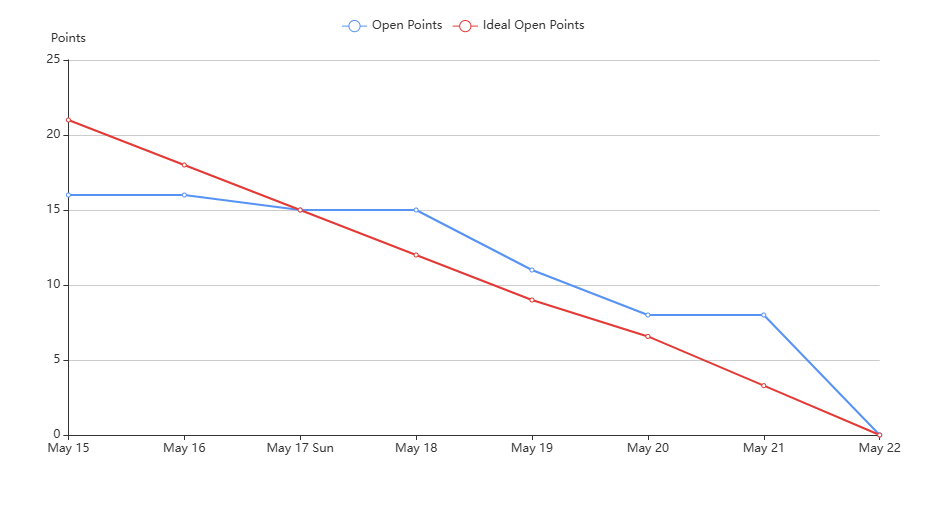
\includegraphics[width=0.7\linewidth]{img/BR_Sprint19}
	\caption[Burndown Report del Sprint 19]{Burndown Report del Sprint 19.}
	\label{fig:brsprint19}
\end{figure}

Como se observa en la Figura~\ref{fig:brsprint19}, el avance del \textit{sprint} fue irregular. Comencé adelantando a la línea ideal, ya que el mismo día del inicio del sprint cerré varias de las issues que estimé ese mismo día, pero se mantuvo firme un buen tiempo, ya que me encontraba en periodo de exámenes y me volvió a superar. Más adelante, sí que logré ponerme más al día y, en la parte final se aprecia un descenso más pronunciado, coincidiendo con el cierre de los ajustes principales y la resolución del \textit{bug} de Selenium, aunque algunas tareas importantes tuvieron que trasladarse al \textit{sprint} siguiente.

\subsection{Sprint 20 - Cierre de la memoria y bugs}
El \textit{Sprint 20} se desarrolló del 23 de mayo al 1 de junio. Para este \textit{sprint} estimé una dedicación inicial de 27~horas, aunque finalmente invertí aproximadamente 29~horas y 30~minutos. El objetivo principal de esta iteración fue avanzar de forma decidida hacia el cierre de la memoria y de los anexos, al mismo tiempo que se resolvían varios \textit{bugs} detectados en la aplicación. A diferencia de otros \textit{sprints}, en este caso conseguí cerrar todas las \textit{issues} dentro del periodo planificado.

Los objetivos definidos para este \textit{sprint} fueron los siguientes:
\begin{itemize}
	\item Redactar el manual del usuario.
	\item Redactar el estudio de viabilidad económica.
	\item Redactar la viabilidad legal.
	\item Redactar el manual del programador.
	\item Redactar la conclusión y las líneas futuras.
	\item Crear el diagrama de interacción general de la aplicación.
	\item Crear el diagrama de secuencia del administrador.
	\item Arreglar la gestión de modelos.
	\item Crear un fichero \texttt{README.md} con un formato más profesional.
	\item Corregir un \textit{bug} de imagen persistente entre diferentes \textit{logins} de sesión.
	\item Realizar ajustes generales en memoria y anexos.
	\item Corregir un \textit{bug} de reescalado y dibujado de trazas (surgió a mitad de sprint).
	\item Arreglar el manual del programador en anexos.
\end{itemize}

En primer lugar, retomé dos tareas que venían parcialmente iniciadas del \textit{sprint} anterior: la redacción del manual del programador y la creación del diagrama de interacción general de la aplicación. En esta iteración ya pude cerrarlas correctamente, al disponer de una versión mucho más estable del sistema y de una visión más clara de los flujos principales. Además, creé el diagrama de secuencia del administrador, con el objetivo de documentar de forma específica las interacciones asociadas a las funcionalidades de gestión.

Una parte importante del \textit{sprint} estuvo dedicada a la redacción de documentación final. Elaboré el manual del usuario, orientado a explicar el funcionamiento de la aplicación desde una perspectiva práctica, y redacté también el estudio de viabilidad económica y la viabilidad legal. Estos apartados eran necesarios para completar la memoria con una visión más global del proyecto, no solo desde el punto de vista técnico, sino también desde su posible uso, mantenimiento y encaje normativo. Asimismo, redacté la conclusión y las líneas futuras, sintetizando el trabajo realizado y dejando planteadas posibles mejoras o ampliaciones posteriores.

En paralelo, realicé varios ajustes en memoria y anexos para mantener la coherencia entre la documentación y el estado real de la aplicación. Dentro de esta revisión, corregí también aspectos del manual del programador en anexos, afinando su estructura y completando explicaciones que habían quedado demasiado esquemáticas.

En cuanto a la aplicación, resolví distintos \textit{bugs} y mejoras funcionales. Por un lado, corregí un problema de imagen persistente entre distintas sesiones, que podía provocar que se mostrase información visual asociada a un usuario anterior. Por otro, solucioné un \textit{bug} relacionado con el reescalado y el dibujado de trazas, ya que afectaba a la correcta representación de los resultados sobre la imagen. Este apareció a mitad de sprint, por lo que es un añadido. Además, arreglé la gestión de modelos, reforzando el comportamiento del panel correspondiente y evitando inconsistencias en su uso.

Finalmente, creé un fichero \texttt{README.md} con un formato más profesional, incorporando una presentación más clara del proyecto, sus funcionalidades principales y la forma de ponerlo en marcha. Con ello, el repositorio quedó más preparado para ser revisado o utilizado por terceros.

\begin{figure}
	\centering
	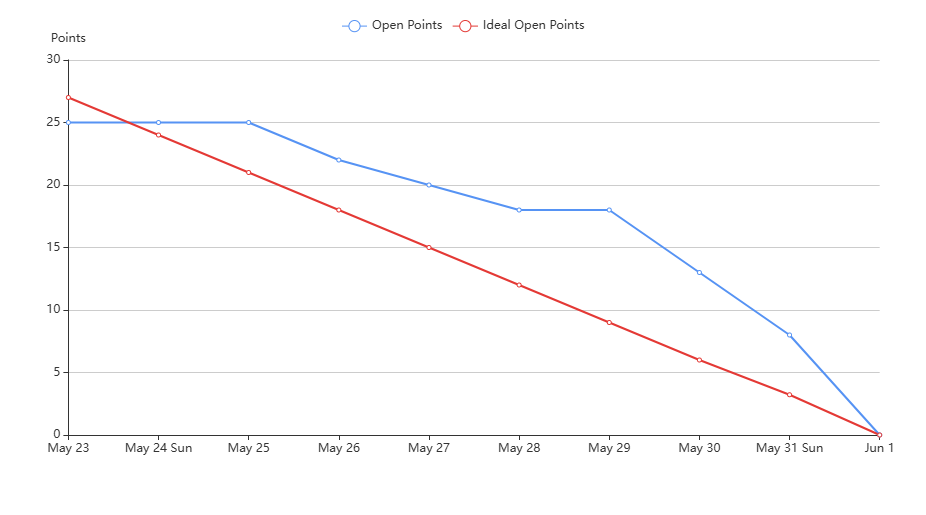
\includegraphics[width=0.7\linewidth]{img/BR_Sprint20}
	\caption[Burndown Report del Sprint 20]{Burndown Report del Sprint 20.}
	\label{fig:brsprint20}
\end{figure}

Como se observa en la Figura~\ref{fig:brsprint20}, el \textit{burndown} muestra un avance progresivo durante todo el \textit{sprint}. Aunque en los primeros días la línea de \textit{open points} se mantuvo algo por encima de la ideal, debido a que varias tareas de documentación requerían trabajo acumulado antes de poder cerrarse, el descenso se fue estabilizando conforme se completaron los principales apartados de memoria y anexos. En la parte final del \textit{sprint} se aprecia una bajada más marcada, coincidiendo con los días en los que acabé los exámenes finales, hasta completar todas las \textit{issues} el 1 de junio.

\subsection{Sprint 21 - Despliegue y mejoras de calidad}
El \textit{Sprint 21} se desarrolló del 2 al 8 de junio. Inicialmente estimé una dedicación de 27,5~horas, aunque durante el avance del \textit{sprint} surgieron nuevas \textit{issues} que elevaron la planificación total a 31,5~horas. Finalmente, la dedicación real fue de aproximadamente 32~horas. El objetivo principal de esta iteración fue realizar el despliegue de la aplicación, cerrar documentación técnica asociada al mismo y corregir distintas incidencias detectadas tanto en el servidor como en el análisis de calidad de SonarQube.

Los objetivos definidos para este \textit{sprint} fueron los siguientes:
\begin{itemize}
	\item Montar Docker para el servidor.
	\item Ejecutar el despliegue de la aplicación.
	\item Arreglar el fichero \texttt{README.md}.
	\item Redactar el tema de la licencia y crear el fichero \texttt{LICENSE.md}.
	\item Cambiar todos los cuadros de comandos de la memoria.
	\item Añadir los últimos \textit{tests} de Selenium y documentarlos.
	\item Incorporar Selenium, Docker, Gunicorn y SonarQube en el apartado de herramientas.
	\item Redactar todo lo referente a Gunicorn y despliegue que todavía faltaba.
	\item Arreglar las tablas de anexos.
	\item Corregir problemas de SonarQube:
	\begin{itemize}
		\item \textit{Security Snapshots}.
		\item \textit{Reliability}.
		\item \textit{Security Hotspots}.
	\end{itemize}
	\item Resolver las nuevas incidencias surgidas durante el \textit{sprint}:
	\begin{itemize}
		\item Arreglar un \textit{bug} de concurrencia en despliegue.
		\item Arreglar el uso de GPU en el servidor.
		\item Permitir iniciar sesión con usuario o correo electrónico.
		\item Informar al usuario cuando no haya seleccionado dos puntos.
	\end{itemize}
\end{itemize}

El primer día del \textit{sprint}, 2 de junio, lo dediqué a preparar la base del despliegue. En primer lugar, monté Docker para el servidor, dejando preparada la infraestructura necesaria para ejecutar la aplicación en el servidor, con el que también empecé a hacer avances. Además, arreglé el fichero \texttt{README.md}.

El 3 de junio cerré tareas de documentación y pruebas. Por un lado, arreglé las tablas de anexos para mantener un formato coherente. Por otro, añadí los últimos \textit{tests} de Selenium y los documenté, completando así la parte de pruebas funcionales sobre la interfaz.

El 4 de junio fue uno de los días más importantes del \textit{sprint}, ya que terminé de ejecutar el despliegue de la aplicación. Durante este proceso también redacté el apartado relativo a la licencia y creé el fichero \texttt{LICENSE.md}. Además, incorporé Selenium, Docker, Gunicorn y SonarQube en el apartado de herramientas de la memoria, para que la documentación reflejase correctamente las tecnologías finalmente utilizadas. Ese mismo día surgieron dos incidencias no previstas: un problema con el uso de la GPU en el servidor y un \textit{bug} de concurrencia durante el despliegue. Ambas incidencias tuvieron que resolverse dentro del propio \textit{sprint}, ya que afectaban directamente al correcto funcionamiento de la aplicación desplegada.

El 5 de junio me centré en la memoria, cambiando todos los cuadros de comandos para homogeneizar su presentación y redactando las partes que todavía faltaban sobre Gunicorn y el despliegue. Esta documentación era necesaria para explicar correctamente cómo se había preparado el entorno de ejecución y qué papel desempeñaba cada componente dentro del servidor.

El 6 de junio incorporé dos mejoras funcionales surgidas durante el avance del \textit{sprint}. La primera consistió en permitir que el usuario pudiese iniciar sesión tanto con su nombre de usuario como con su correo electrónico, haciendo el acceso más flexible. La segunda fue añadir un aviso cuando el usuario no hubiese seleccionado dos puntos en el visor, evitando así errores silenciosos y mejorando la retroalimentación de la interfaz.

Finalmente, los días 7 y 8 de junio los dediqué principalmente a resolver incidencias detectadas por SonarQube. El día 7 corregí problemas asociados a \textit{Security Snapshots} y \textit{Reliability}, mientras que el día 8 cerré los \textit{Security Hotspots}. Con ello, el proyecto quedó en un estado más limpio desde el punto de vista de calidad de código y análisis estático.

\begin{figure}
	\centering
	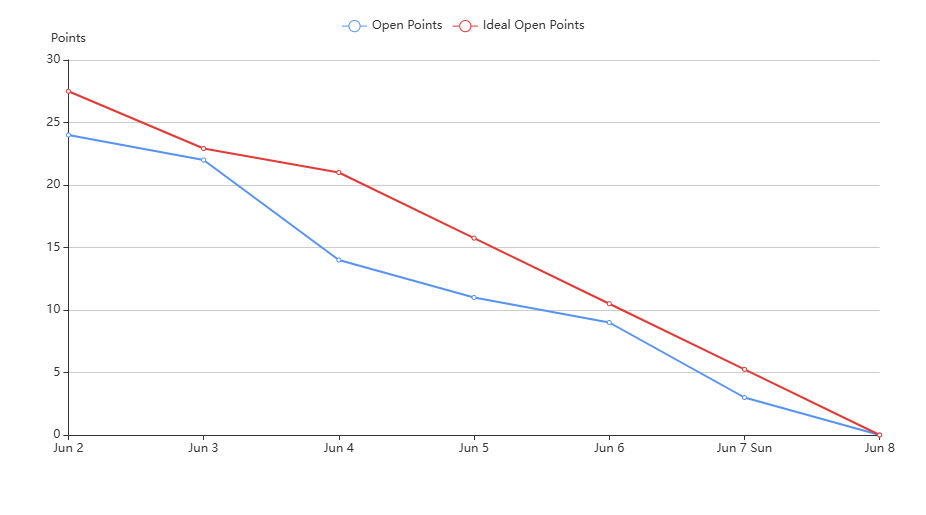
\includegraphics[width=0.7\linewidth]{img/BR_Sprint21}
	\caption[Burndown Report del Sprint 21]{Burndown Report del Sprint 21.}
	\label{fig:brsprint21}
\end{figure}

Como se observa en la Figura~\ref{fig:brsprint21}, el \textit{burndown} muestra un avance bastante constante durante todo el \textit{sprint}, adelantando ya el primer día a la línea ideal, debido a que cerré varias de las issues planificadas ese mismo día. Aunque surgieron varias tareas nuevas durante la semana, especialmente relacionadas con el despliegue y con incidencias del servidor, estas se fueron resolviendo dentro del propio periodo. La línea de \textit{open points} se mantuvo siempre por debajo de la ideal, reflejando que el cierre de tareas fue progresivo y que el \textit{sprint} pudo completarse correctamente el 8 de junio.

\section{Estudio de viabilidad}
En este apartado se analiza la viabilidad del proyecto desde una doble perspectiva: económica, valorando los costes asociados a su desarrollo, despliegue y mantenimiento; y legal, revisando las licencias, condiciones de uso y obligaciones normativas que afectan a las tecnologías, datos y recursos empleados.

\subsection{Viabilidad económica}

En este apartado se realiza una estimación económica del proyecto, considerando los principales recursos necesarios para su desarrollo, puesta en marcha y mantenimiento básico. Aunque el trabajo se ha realizado en un contexto académico y no persigue una explotación comercial inmediata, resulta conveniente valorar su coste aproximado como si fuese desarrollado dentro de un entorno profesional. Para ello, se tienen en cuenta los costes de personal, hardware, software, despliegue, mantenimiento e indirectos, así como los beneficios no económicos derivados de la aplicación.

La duración total del proyecto ha sido de, aproximadamente, siete meses y medio. Para el escenario base se toma como referencia un perfil de desarrollador \textit{full-stack} junior avanzado, con conocimientos de Python, Flask, pruebas automáticas e integración de modelos de inferencia. Se considera un salario bruto anual de \num{30000}\,€, situado entre las referencias salariales de un perfil junior Python y un perfil Python/Django en España, y ajustado al tipo de responsabilidades asumidas durante el desarrollo~\cite{glassdoor_python_developer_spain_2026}.

\subsubsection{Costes de personal}

El coste de personal constituye la partida principal del proyecto, ya que la mayor parte del esfuerzo se ha concentrado en el análisis del problema, el estudio del algoritmo base, el desarrollo de la aplicación web, la integración de la inferencia, la implementación del visor cartográfico, la gestión de usuarios y modelos, las pruebas y la documentación.

Para el cálculo del coste por hora se emplean las siguientes expresiones:

\begin{equation}
	\text{Coste bruto por hora} =
	\frac{\text{Salario bruto anual}}{\num{1760}}
\end{equation}

\begin{equation}
	\text{Coste empresa por hora} =
	\text{Coste bruto por hora} \times (1 + \num{0.3057})
\end{equation}

\begin{equation}
	\text{Coste de desarrollo} =
	\text{Horas dedicadas} \times \text{Coste empresa por hora}
\end{equation}

El factor \num{0.3057} representa una aproximación a las cotizaciones empresariales a la Seguridad Social, considerando contingencias comunes, desempleo, FOGASA, formación profesional y MEI~\cite{seguridad_social_bases_tipos_cotizacion_2026}.

En la tabla~\ref{tab:cotizaciones_empresa} se resumen los porcentajes considerados para estimar el sobrecoste empresarial aplicado al salario bruto.

\begin{table}[]
	\centering
	\renewcommand{\arraystretch}{1.25}
	
	\begin{tabular}{l r}
		\toprule
		\textbf{Concepto} & \textbf{Porcentaje} \\
		\midrule
		Contingencias comunes & \qty{23.60}{\percent} \\
		Desempleo & \qty{5.50}{\percent} \\
		FOGASA & \qty{0.20}{\percent} \\
		Formación profesional & \qty{0.60}{\percent} \\
		MEI & \qty{0.67}{\percent} \\
		\midrule
		\textbf{Total aproximado} & \textbf{\qty{30.57}{\percent}} \\
		\bottomrule
	\end{tabular}
	
	\caption{Distribución aproximada de cotizaciones empresariales aplicadas al coste de personal.}
	\label{tab:cotizaciones_empresa}
\end{table}

En el caso del desarrollador principal, se estima una dedicación aproximada de \num{21} semanas, con una media de \num{23} horas semanales, lo que supone un total de \num{483} horas de trabajo. Para la labor de supervisión se considera una dedicación de \num{30} horas por cada tutor, asociada a reuniones, revisión de avances, orientación técnica y seguimiento del proyecto.

La Tabla~\ref{tab:costes_personal} recoge la estimación de horas y costes asociados al desarrollador principal y a las labores de supervisión del proyecto.

\begin{table}[]
	\centering
	\small
	\renewcommand{\arraystretch}{1.25}
	\setlength{\tabcolsep}{5pt}
	\begin{tabular}{p{4.0cm} p{2.8cm} r r r}
		\toprule
		\textbf{Persona} & \textbf{Rol} & \textbf{Horas} & \textbf{Coste/h (€)} & \textbf{Coste (€)} \\
		\midrule
		Marcos Zamorano Lasso & Desarrollador & \num{483} & \num{22.26} & \num{10749.77} \\
		Álvar Arnaiz González & Supervisor & \num{30} & \num{33.38}\ & \num{1001.53} \\
		David Martínez Acha & Supervisor & \num{30} & \num{33.38} & \num{1001.53} \\
		\midrule
		\textbf{Total} & & \textbf{\num{543}} & & \textbf{\num{12752.83}} \\
		\bottomrule
	\end{tabular}
	\caption{Estimación de costes de personal del proyecto.}
	\label{tab:costes_personal}
\end{table}


\subsubsection{Costes de hardware}

Para el desarrollo del proyecto se ha utilizado un equipo portátil personal, suficiente para implementar la aplicación, ejecutar el entorno Flask, realizar pruebas locales y llevar a cabo inferencias de validación. Aunque no ha sido necesario adquirir hardware específico, se imputa una parte proporcional del coste del equipo en función de su vida útil estimada.

El coste de hardware se calcula mediante la expresión:

\begin{equation}
	\text{Coste hardware} =
	\frac{\text{Precio del equipo}}{\text{Vida útil}} \times
	\frac{\text{Meses del proyecto}}{\num{12}}
\end{equation}

Considerando un equipo valorado en \num{1200}\,€, una vida útil de \num{5} años y una duración del proyecto de \num{7.5} meses, se obtiene:

\begin{equation}
	\text{Coste hardware} =
	\frac{\num{1200}}{\num{5}} \times \frac{\num{7.5}}{\num{12}}
	= \num{150.00}\,\text{€}
\end{equation}

La tabla~\ref{tab:costes_hardware} muestra el coste de hardware imputado al proyecto según el criterio de amortización descrito.

\begin{table}[]
	\centering
	\renewcommand{\arraystretch}{1.25}
	\begin{tabular}{l r r r}
		\toprule
		\textbf{Elemento} & \textbf{Precio} & \textbf{Vida útil} & \textbf{Coste imputado} \\
		\midrule
		Equipo portátil de desarrollo & \num{1200}\,€ & \num{5} años & \num{150.00}\,€ \\
		\midrule
		\textbf{Total} & & & \textbf{\num{150.00}\,€} \\
		\bottomrule
	\end{tabular}
	\caption{Costes de hardware imputados al proyecto.}
	\label{tab:costes_hardware}
\end{table}

\subsubsection{Costes de software}

En cuanto al software, se ha priorizado el uso de herramientas gratuitas, de código abierto o disponibles sin coste adicional para el desarrollo académico. Esto incluye el lenguaje Python, el \textit{framework} Flask, SQLite, SQLAlchemy, PyTorch, Tailwind CSS, DaisyUI, Leaflet, Git, GitHub, Visual Studio Code, \textit{diagrams.net}, TeXstudio, MiKTeX y Jupyter Notebook, entre otras herramientas utilizadas durante el desarrollo y la documentación.

No obstante, sí que se imputa un coste estimado de licencia Windows, tomando como referencia el coste habitual de una licencia de sistema operativo de escritorio. Este valor podría variar según el tipo de licencia, canal de compra o inclusión previa en el equipo~\cite{xataka_windows10_licencias_precios_2020}.

La tabla~\ref{tab:costes_software} recoge los costes de software considerados en el proyecto.

\begin{table}[]
	\centering
	\small
	\renewcommand{\arraystretch}{1.25}
	\begin{tabular}{p{4cm} p{7cm} r}
		\toprule
		\textbf{Software} & \textbf{Uso principal} & \textbf{Coste} \\
		\midrule
		Python, Flask y extensiones & Desarrollo de la aplicación web y backend & \num{0.00}\,€ \\
		PyTorch y librerías de inferencia & Ejecución de modelos de segmentación & \num{0.00}\,€ \\
		SQLite y SQLAlchemy & Persistencia y acceso a datos & \num{0.00}\,€ \\
		Tailwind CSS, DaisyUI y Leaflet & Interfaz web y visor cartográfico & \num{0.00}\,€ \\
		Git, GitHub y Zube & Control de versiones y gestión del proyecto & \num{0.00}\,€ \\
		TeXstudio, MiKTeX y diagrams.net & Documentación y diagramas & \num{0.00}\,€ \\
		Visual Studio Code y Jupyter Notebook & Desarrollo, pruebas y análisis del algoritmo & \num{0.00}\,€ \\
		Licencia Windows & Sistema operativo utilizado durante el desarrollo & \num{145.00}\,€ \\
		\midrule
		\textbf{Total} & & \textbf{\num{145.00}\,€} \\
		\bottomrule
	\end{tabular}
	\caption{Costes de software considerados en el proyecto.}
	\label{tab:costes_software}
\end{table}

Por tanto, el coste directo de software asciende a \num{145.00}\,€. La mayor parte de las herramientas utilizadas no han requerido pagos adicionales durante el desarrollo del TFG, al tratarse de tecnologías gratuitas, libres o disponibles sin coste para un uso académico.

\subsubsection{Costes de despliegue y mantenimiento}

Aunque la aplicación puede ejecutarse en local durante el desarrollo y se despliega en una infraestructura universitaria, se estima un escenario de referencia basado en un despliegue básico en un servidor privado virtual, tomando como referencia precios habituales de proveedores de servidores cloud~\cite{hetzner_cloud_cx_plans_2024}. Este escenario permite aproximar el coste que tendría mantener la aplicación disponible durante el periodo equivalente al desarrollo.

Además del alojamiento, debe considerarse una dedicación mensual de mantenimiento para tareas como actualización de dependencias, revisión de logs, copias de seguridad, limpieza de ficheros generados y supervisión del servicio mediante Gunicorn. Se estima una dedicación media de \num{1.5} horas mensuales durante \num{7.5} meses.

En la tabla~\ref{tab:costes_despliegue} se recoge una estimación de estos costes descritos.

\begin{table}[]
	\centering
	\renewcommand{\arraystretch}{1.25}
	\begin{tabular}{p{5cm} r r r}
		\toprule
		\textbf{Concepto} & \textbf{Coste unitario} & \textbf{Periodo} & \textbf{Coste} \\
		\midrule
		Servidor VPS básico & \num{12.00}\,€/mes & \num{7.5} meses & \num{90.00}\,€ \\
		Dominio web & \num{12.00}\,€/año & \num{7.5} meses & \num{7.50}\,€ \\
		Almacenamiento y copias de seguridad & \num{5.00}\,€/mes & \num{7.5} meses & \num{37.50}\,€ \\
		Mantenimiento técnico & \num{22.26}\,€/h & \num{11.25} h & \num{250.38}\,€ \\
		\midrule
		\textbf{Total} & & & \textbf{\num{385.38}\,€} \\
		\bottomrule
	\end{tabular}
	\caption{Estimación de costes de despliegue y mantenimiento.}
	\label{tab:costes_despliegue}
\end{table}

\subsubsection{Costes indirectos}

Además de los costes directos, se consideran costes indirectos asociados al desarrollo del proyecto. En esta categoría se incluyen gastos como electricidad, conexión a internet, infraestructura doméstica o universitaria, material auxiliar y otros recursos de apoyo no imputados de forma individual.

Siguiendo una estimación habitual en este tipo de estudios, se aplica un \qty{15}{\percent} sobre el total de costes directos:

\begin{equation}
	\text{Costes indirectos} =
	\text{Costes directos} \times \num{0.15}
\end{equation}

La Tabla~\ref{tab:costes_totales} resume el coste económico total estimado del proyecto, incorporando tanto costes directos como costes indirectos.

\begin{table}[]
	\centering
	\renewcommand{\arraystretch}{1.25}
	\begin{tabular}{l r}
		\toprule
		\textbf{Tipo de coste} & \textbf{Importe (€)} \\
		\midrule
		Costes de personal & \num{12752.83} \\
		Costes de hardware & \num{150.00} \\
		Costes de software & \num{145.00} \\
		Costes de despliegue y mantenimiento & \num{385.38} \\
		\midrule
		Costes directos & \num{13433.21} \\
		Costes indirectos, \qty{15}{\percent} & \num{2014.98} \\
		\midrule
		\textbf{Coste total estimado} & \textbf{\num{15448.19}} \\
		\bottomrule
	\end{tabular}
	\caption{Resumen de costes económicos del proyecto.}
	\label{tab:costes_totales}
\end{table}

\subsubsection{Beneficios}

No se esperan ingresos comerciales directos derivados del proyecto, ya que su finalidad es puramente académica e investigadora. La aplicación se ha concebido como un prototipo funcional orientado a demostrar la viabilidad de integrar modelos de segmentación semántica en un entorno web accesible, no como un producto comercial cerrado.

No obstante, sí existen beneficios intangibles relevantes. En primer lugar, el sistema puede servir como apoyo a investigaciones relacionadas con el análisis de trazas de herbivoría y presión ecológica. Adicionalmente, automatiza parcialmente una tarea que, de forma manual, resultaría costosa, lenta y difícil de escalar.

\subsubsection{Conclusión}

Desde el punto de vista económico, el proyecto resulta viable en un contexto académico, principalmente porque se ha apoyado en herramientas gratuitas, bibliotecas de código abierto y recursos hardware ya disponibles. La partida más relevante corresponde al coste de personal, algo esperable en un proyecto software donde el mayor valor se encuentra en el análisis, diseño, implementación, pruebas y documentación.

El coste total estimado asciende a \num{15448.19}\,€, considerando personal, hardware, software, despliegue, mantenimiento e indirectos. Aunque no se prevén beneficios comerciales directos, el proyecto aporta valor investigador, académico y técnico, además de constituir una base sólida para futuras líneas de desarrollo relacionadas con la monitorización ecológica mediante imágenes aéreas y modelos de visión por computador.

\subsection{Viabilidad legal}

En este apartado se analiza la viabilidad legal del proyecto, atendiendo a los aspectos que condicionan su desarrollo, uso y despliegue en un entorno universitario. Para ello, se revisan las licencias del software empleado, las condiciones de uso de las fuentes cartográficas, la situación específica de Google Earth Engine, el tratamiento de datos personales, la gestión de imágenes subidas por los usuarios, la incorporación de modelos de segmentación y las obligaciones básicas de accesibilidad. 

El objetivo de este estudio no es realizar una auditoría jurídica exhaustiva, sino identificar los principales riesgos legales y comprobar que la solución planteada puede utilizarse en un contexto académico siempre que se respeten las condiciones de uso aplicables.

\subsubsection{Licencias de software}

La aplicación se ha desarrollado principalmente mediante herramientas, bibliotecas y \textit{frameworks} de código abierto. En general, las licencias utilizadas son de carácter permisivo, como MIT, BSD o Apache-2.0, lo que permite su uso, modificación y redistribución en proyectos académicos y de investigación, siempre que se conserven los avisos de copyright y licencia correspondientes.

La Tabla~\ref{tab:licencias_software} recoge las principales dependencias y herramientas utilizadas, junto con la licencia asociada a cada una de ellas.

\begin{table}[]
	\centering
	\small
	\renewcommand{\arraystretch}{1.15}
	
	\begin{tabularx}{\textwidth}{@{}
			>{\RaggedRight\arraybackslash}X
			c
			>{\RaggedRight\arraybackslash}X
			@{}}
		\toprule
		\textbf{Librería} & \textbf{Versión} & \textbf{Licencia} \\
		\midrule
		\textit{Python} & 3.12 & PSF \\
		\textit{Flask} & 3.1.2 & BSD-3 \\
		\textit{SQLAlchemy} & 2.0.49 & MIT \\
		\textit{SQLite} & 3.45.0 & Dominio público \\
		\textit{Jinja2} & 3.1.6 & BSD-3 \\
		\textit{Tailwind CSS} & 3.4.17 & MIT \\
		\textit{DaisyUI} & 4.12.24 & MIT \\
		\textit{Selenium} & 4.38.0 & Apache-2.0 \\
		\textit{Pytest} & 9.0.1 & MIT \\
		\textit{Coverage.py} & 7.13.5 & Apache-2.0 \\
		\textit{PyTorch} & 2.10.0 & BSD-style \\
		\textit{Segmentation Models PyTorch} & 0.5.0 & MIT \\
		\textit{Timm} & 1.0.24 & Apache-2.0 \\
		\textit{Hugging Face Hub} & 1.3.4 & Apache-2.0 \\
		\textit{ReportLab} & 4.5.0 & BSD \\
		\textit{Gunicorn} & 23.0.0 & MIT \\
		\textit{SonarQube Community Build} & 25.4 & LGPLv3 / SSAL v1.0 \\
		\bottomrule
	\end{tabularx}
	
	\caption{Bibliotecas usadas, versiones y licencias.}
	\label{tab:licencias_software}
\end{table}

Para seleccionar la licencia del proyecto se ha partido del análisis de las dependencias empleadas y de sus condiciones de uso, resumidas previamente en la Tabla~\ref{tab:licencias_software}. La mayoría de las tecnologías utilizadas se distribuyen bajo licencias permisivas, principalmente MIT, BSD-3-Clause y Apache-2.0, lo que permite su uso en un contexto académico siempre que se respeten los avisos de copyright, las condiciones de redistribución y las obligaciones particulares de cada biblioteca. No obstante, al combinar distintas dependencias, resulta conveniente adoptar una licencia que no solo sea permisiva, sino que también cubra de forma clara las exigencias más completas presentes en el ecosistema utilizado.

En este sentido, se ha descartado emplear una licencia excesivamente simple, como MIT, como licencia principal del proyecto, no porque sea incompatible con el desarrollo realizado, sino porque podría resultar insuficiente para reflejar algunas obligaciones presentes en dependencias más específicas. En particular, bibliotecas y herramientas del ámbito de aprendizaje profundo y modelos, como \texttt{timm} o componentes asociados al ecosistema de Hugging Face, utilizan licencias como Apache-2.0, que incorporan aspectos adicionales, entre ellos la concesión expresa de derechos de patente y la obligación de indicar modificaciones cuando proceda. Por tanto, para garantizar una mayor coherencia jurídica con las dependencias empleadas y evitar ambigüedades en la reutilización futura del código, se ha optado por publicar el proyecto bajo la licencia \textbf{Apache License 2.0}.

La elección de Apache-2.0 resulta especialmente adecuada para este Trabajo Fin de Grado, ya que el proyecto se apoya de forma importante en técnicas de visión por computador, inferencia con modelos de segmentación y bibliotecas propias del ecosistema de \textit{deep learning}. Esta licencia permite el uso privado, académico y comercial del software, así como su modificación y redistribución, siempre que se incluya una copia de la licencia, se mantengan los avisos de copyright y se indiquen de forma clara las modificaciones realizadas sobre los archivos originales. Además, incorpora una concesión expresa de derechos de patente, aspecto relevante en proyectos que implementan o integran algoritmos de análisis de imágenes. Finalmente, la licencia limita la responsabilidad del autor frente a posibles daños derivados del uso del software, lo que resulta adecuado para un proyecto académico que puede servir como base para futuros desarrollos o investigaciones.

\subsubsection{Licencias de datos cartográficos}

La aplicación contempla el uso de ortofotografía aérea procedente del Plan Nacional de Ortofotografía Aérea, gestionado por el IGN y el CNIG. Este tipo de datos puede utilizarse de forma libre y gratuita bajo una licencia compatible con CC-BY 4.0, siempre que se reconozca adecuadamente el origen y la propiedad de la información geográfica~\cite{cnig_pnoa_maxima_actualidad,pnoa_ign}.

Por tanto, el uso de PNOA resulta legalmente adecuado, siempre que se incluya una atribución clara a IGN, CNIG y PNOA en la documentación, en la memoria y, también, en la interfaz de usuario cuando se muestren capas o imágenes procedentes de dichos servicios. Esta atribución permite cumplir con las condiciones de reconocimiento de autoría y refuerza la trazabilidad de los datos utilizados.

\subsubsection{Google Earth Engine}

Google Earth Engine sería la plataforma más adecuada para el análisis geoespacial de este proyecto, pero actualmente no se dispone de una licencia o acceso formal integrado en el mismo. Por este motivo, no debe presentarse como una dependencia actual del sistema ni utilizarse en producción sin autorización adecuada~\cite{googleearthengine_terms}.

En caso de que en el futuro la Universidad de Burgos obtuviera acceso institucional, Google Earth Engine podría incorporarse como una mejora relevante del sistema, especialmente para acceder a fuentes de imaginería más próximas a aquellas empleadas durante el entrenamiento del modelo. Sin embargo, dicha integración debería respetar estrictamente sus términos de uso, incluyendo el empleo de una cuenta institucional, la finalidad académica o no comercial cuando corresponda y la revisión periódica del acceso por parte de Google~\cite{googleearthengine_terms}.

Además, si el uso evolucionase hacia un contexto comercial, operacional o de explotación sostenida, habría que considerar los planes de pago disponibles. Según la información de precios de Google Cloud, los planes comerciales de Earth Engine incluyen cuotas mensuales de 500 USD para el plan Basic y 2.000 USD para el plan Professional~\cite{googleearthengine_pricing}. Por ello, cualquier uso futuro deberá analizarse tanto desde la perspectiva técnica como desde la económica y contractual.

\subsubsection{Protección de datos personales}

La aplicación trata datos personales de los usuarios, como nombre de usuario, correo electrónico, teléfono, contraseña hasheada, rol, fecha de alta, imagen de perfil, imágenes subidas y colecciones geoespaciales asociadas a una cuenta. En consecuencia, el sistema debe ajustarse al Reglamento General de Protección de Datos y a la Ley Orgánica 3/2018 de Protección de Datos Personales y garantía de los derechos digitales~\cite{rgpd_2016,lopdgdd_2018}.

Desde el punto de vista del diseño, se deben aplicar principios como minimización de datos, limitación de finalidad, control de acceso y seguridad por defecto. La aplicación ya incorpora autenticación, roles de usuario y separación de permisos, lo que contribuye a restringir el acceso a la información. Asimismo, las contraseñas no deben almacenarse en texto plano, sino mediante funciones de \textit{hash} seguras, como las proporcionadas por Werkzeug.

También deben contemplarse los derechos de las personas usuarias, especialmente acceso, rectificación y supresión de sus datos. En la práctica, esto implica que el sistema debería permitir consultar la información asociada a la cuenta, modificar datos básicos del perfil y eliminar, cuando proceda, imágenes, colecciones o recursos vinculados al usuario. Al desplegar el sistema en servidores de la Universidad de Burgos, se aplican además las políticas internas de seguridad, alojamiento, copias de seguridad y conservación de datos.

\subsubsection{Imágenes subidas por usuarios}

Las imágenes subidas por los usuarios pueden contener información sensible o estar sujetas a derechos de terceros. Por ello, la aplicación debe asumir que el usuario es responsable de disponer de los derechos necesarios para cargar y procesar dichas imágenes. El sistema debe limitar su uso a la finalidad prevista, es decir, calcular trazas, generar resultados asociados y permitir su visualización o descarga dentro del flujo de la aplicación.

Además, resulta conveniente que la aplicación permita borrar las imágenes y resultados generados, de forma que el usuario pueda retirar del sistema aquellos recursos que ya no desee mantener. Al no guardar la imagen en el sistema hasta que no se pulsa el botón de \textit{Calcular trazas}, evitamos que se guarde una imagen que el usuario haya introducido erróneamente, pudiendo borrarla en cualquier momento sin mayor repercusión.

\subsubsection{Modelos de segmentación}

Los modelos de segmentación y pesos incorporados al sistema pueden estar sujetos a licencias propias. Esto es especialmente relevante cuando se emplean modelos descargados desde repositorios externos, plataformas como Hugging Face o implementaciones que dependan de arquitecturas concretas. Aunque el código de muchas bibliotecas utilizadas sea permisivo, los pesos, \textit{checkpoints} o conjuntos de datos empleados para entrenarlos pueden imponer restricciones adicionales~\cite{huggingface_hub_license}.

Por este motivo, antes de distribuir la aplicación junto con modelos entrenados, o antes de permitir su uso en un entorno más amplio, debe verificarse la licencia de cada artefacto. En el caso de modelos subidos por administradores, el sistema puede validar su compatibilidad técnica, pero la compatibilidad legal debe comprobarse previamente por la persona responsable de su incorporación.

\subsubsection{Despliegue en servidor}

El despliegue en un servidor de la Universidad de Burgos resulta viable desde el punto de vista legal siempre que se respeten las condiciones de uso de las tecnologías empleadas, las licencias de los datos cartográficos y la normativa de protección de datos. Al tratarse de un entorno institucional, la aplicación se ajusta a las políticas de seguridad, acceso, almacenamiento y copias de seguridad establecidas por la universidad.

Asimismo, el despliegue deberá evitar el uso de servicios externos sin licencia adecuada, especialmente en lo relativo a Google Earth Engine o a fuentes cartográficas sujetas a restricciones. En caso de utilizar PNOA como fuente de ortofotografía, será necesario mantener la atribución correspondiente a IGN/CNIG/PNOA y garantizar que las imágenes obtenidas se emplean conforme a sus condiciones de reutilización.

\subsubsection{Accesibilidad}

Al publicarse la aplicación en un entorno universitario o si se integra como servicio accesible desde infraestructura pública, resulta conveniente considerar el Real Decreto 1112/2018, relativo a la accesibilidad de los sitios web y aplicaciones para dispositivos móviles del sector público~\cite{rd1112_2018}. Aunque el proyecto se ha desarrollado como TFG y no como servicio administrativo final, tener en cuenta estos criterios desde el diseño facilita su posible evolución futura.

En este sentido, la aplicación debería procurar una interfaz clara, formularios etiquetados, contraste suficiente, navegación comprensible, textos alternativos cuando proceda y compatibilidad razonable con tecnologías de apoyo. Estas medidas no solo tienen relevancia legal, sino que también mejoran la usabilidad general del sistema para todos los usuarios.

\subsubsection{Conclusión}

Desde el punto de vista legal, el proyecto resulta viable en un entorno académico siempre que se respeten las licencias de las bibliotecas utilizadas, se mantenga la atribución correspondiente a los datos cartográficos del IGN/CNIG/PNOA, se cumpla la normativa de protección de datos y no se utilice Google Earth Engine sin acceso o licencia adecuada.

En conjunto, la solución también es coherente con la viabilidad económica analizada previamente, ya que se apoya en herramientas de bajo coste directo, tecnologías abiertas y un posible despliegue en infraestructura universitaria. No obstante, cualquier evolución hacia un uso público estable, comercial u operacional deberá revisar de nuevo las condiciones de licenciamiento, privacidad, accesibilidad y explotación de datos o modelos.



